% \part{数学建模实战}
% \chapter{系泊系统}

\documentclass[UTF8]{ctexbook}

\ctexset{
    part/number = \chinese{part}
}
\usepackage{multirow}
\usepackage{amsmath}% ams 数学公式
\usepackage{amsfonts}% ams 数学字体
\usepackage{bbm}%重影字体
\usepackage{amssymb,latexsym}% ams 数学符号与LaTeX数学符号
\usepackage{mathrsfs}% 花式符号
\usepackage{ntheorem}%定理、定义、证明
    \theoremstyle{nonumberplain}
    \theoremheaderfont{\bfseries}
    \theorembodyfont{\normalfont}
    \theoremsymbol{$\square$}
    \newtheorem{Proof}{\hskip 2em 证明}
    \newtheorem{theorem}{\hspace{2em}定理}[chapter]
    \newtheorem{definition}{\hspace{2em}定义}[chapter] % 如果没有章, 只有节, 把上面的[chapter]改成[section]
    \newtheorem{axiom}[definition]{\hspace{2em}公理}
    \newtheorem{lemma}[definition]{\hspace{2em}引理}
    \newtheorem{proposition}[definition]{\hspace{2em}命题}
    \newtheorem{corollary}[definition]{\hspace{2em}推论}
    \newtheorem{remark}{\hspace{2em}注}[chapter] %类似地定义其他“题头”. 这里“注”的编号与定义、定理等是分开的
    \newtheorem{Assumption}{\hspace{2em}假设}[chapter]

%算法伪代码
%http://blog.csdn.net/lwb102063/article/details/53046265
\usepackage{algorithm}
\usepackage{algorithmicx}
\usepackage{algpseudocode}
    \floatname{algorithm}{算法}
    \renewcommand{\algorithmicrequire}{\textbf{输入:}}
    \renewcommand{\algorithmicensure}{\textbf{输出:}}
% 罗马数字:示例:\rom{2}
\makeatletter
\newcommand*{\rom}[1]{\expandafter\@slowromancap\romannumeral #1@}
\makeatother

\usepackage{enumerate}%itemiz环境。\begin{enumerate}[step 1][a)]可以使用 A,a,I,i,1 作为可选项产生 \Alph,\alph,\Roman,\roman,\arabic 的效果
\usepackage{cite}%参考文献
    \bibliographystyle{plain}
\usepackage{extarrows}% 带参数的箭头
\usepackage{hyperref}% 超链接
\usepackage{pifont}%然后在正文输入\ding{172}~\ding{211}得到相应数字,要是要①就输入:\ding{172}②就输:\ding{173}
%\usepackage[CJKbookmarks, colorlinks, bookmarksnumbered=true,pdfstartview=FitH,linkcolor=black,citecolor=black]{hyperref}%超链接的格式设置
\hypersetup{
    colorlinks=false,% 去掉超链接颜色
    pdfborder=0 0 0% 取消超链接的边框
}
\usepackage{graphicx}% 图片管理
\usepackage{caption}
\usepackage{subcaption}%并排的图各有标题
\graphicspath{{images/}}% 设置图片搜索路径
\usepackage{float,varwidth}% 浮动体
\usepackage{booktabs}% 三线表
\usepackage{fancyhdr}% 页眉设置
\usepackage{xcolor}% 颜色宏包
\usepackage{colortbl}% 彩色表格
\usepackage{listings}% 代码高亮
\usepackage{caption}% 对标题进行控制,如让\caption标题的字体缩小一号,同时数字标签使用粗体可以用:\usepackage[font=small,labelfont=bf]{caption}
\usepackage{xfrac,upgreek}%分别是行间公式如a/b的形式(将原来的命令\frac改成\sfrac)和希腊字体的宏包的
\usepackage{mathtools}%lgathered和rgathered环境把公式向左向右对齐
\usepackage{tabularx}%提供自动延伸的表列,(X列格式说明符),文字过长时可以自动转行
\usepackage{longtable}%长表格
\usepackage{enumitem}%enumerate宏包的升级
\usepackage{harpoon}%数学公式的矢量
\usepackage{bookmark}%目录的书签
\renewcommand{\headwidth}{\textwidth}%图片并排,这个要列在所有宏包的后面
\definecolor{codegreen}{rgb}{0,0.6,0}
\definecolor{codegray}{rgb}{0.5,0.5,0.5}
\definecolor{codepurple}{rgb}{0.58,0,0.82}
\definecolor{backcolour}{rgb}{0.95,0.95,0.92}
\lstset{
    commentstyle=\color{codegreen},
    keywordstyle=\color{magenta},
    numberstyle=\tiny\color{codegray},
    stringstyle=\color{codepurple},
    basicstyle=\footnotesize,
    breakatwhitespace=false,% 断行只在空格处
    breaklines=true,% 自动断行
    captionpos=b,% 标题位置
    keepspaces=true,
    numbers=left,
    numbersep=5pt,
    showspaces=false,
    showstringspaces=false,
    showtabs=false,% 显示
    tabsize=2% TAB 被当作两个空格
}
\topmargin=0pt\oddsidemargin=0pt\evensidemargin=0pt
\textwidth=16.5cm\textheight=23cm\raggedbottom%我这么设置是为了缩小页边距,满足有的文字无法转行
\pagestyle{headings}%页眉为章节标题,无页脚
\setlength{\abovecaptionskip}{10pt}
\setlength{\belowcaptionskip}{-15pt}%图片表格的前后距离设置
\CTEXsetup[format={\zihao{-3}\raggedright\bfseries}]{section}%设置节的格式

\begin{document}
% \part{数学建模实战}
\chapter{系泊系统}
\section{题目要求}
    \par
    近浅海观测网的传输节点由浮标系统、系泊系统和水声通讯系统组成,如图(\ref{fig:系泊系统组成图})所示。1、某型传输节点的浮标系统可简化为底面直径$2m$、高$2m$的圆柱体,浮标的质量为$1000kg$。2、系泊系统由钢管、钢桶、重物球、电焊锚链和特制的抗拖移锚组成。锚的质量为$600kg$,锚链选用无档普通链环,近浅海观测网的常用型号及其参数在附表中列出。钢管共4节,每节长度$1m$,直径为$50mm$,每节钢管的质量为$10kg$。要求锚链末端与锚的链接处的切线方向与海床的夹角不超过16度,否则锚会被拖行,致使节点移位丢失。3、水声通讯系统安装在一个长$1m$、外径$30cm$的密封圆柱形钢桶内,设备和钢桶总质量为$100kg$。钢桶上接第4节钢管,下接电焊锚链。钢桶竖直时,水声通讯设备的工作效果最佳。若钢桶倾斜,则影响设备的工作效果。钢桶的倾斜角度(钢桶与竖直线的夹角)超过5度时,设备的工作效果较差。为了控制钢桶的倾斜角度,钢桶与电焊锚链链接处可悬挂重物球。
            \begin{figure}[H]
            \centering
            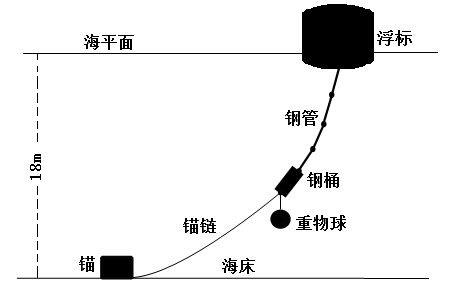
\includegraphics[height=4cm]{images/xiposystem.jpg}
            \caption{系泊系统组成图}
            \label{fig:系泊系统组成图}
            \end{figure}
    \par
    系泊系统的设计问题就是确定锚链的型号、长度和重物球的质量,使得浮标的吃水深度和游动区域及钢桶的倾斜角度尽可能小。
    \par
    \textbf{问题1}:某型传输节点选用II型电焊锚链$22.05m$,选用的重物球的质量为$1200kg$。现将该型传输节点布放在水深$18m$、海床平坦、海水密度为$1.025\times 10^3kg/m^3$的海域。若海水静止,分别计算海面风速为$12m/s$和$24m/s$时钢桶和各节钢管的倾斜角度、锚链形状、浮标的吃水深度和游动区域。
    \par
    \textbf{问题2}:在问题1的假设下,计算海面风速为$36m/s$时钢桶和各节钢管的倾斜角度、锚链形状和浮标的游动区域。请调节重物球的质量,使得钢桶的倾斜角度不超过5度,锚链在锚点与海床的夹角不超过16度。
    \par
    \textbf{问题3}:由于潮汐等因素的影响,布放海域的实测水深介于$16m~20m$之间。布放点的海水速度最大可达到$1.5m/s$、风速最大可达到$36m/s$。请给出考虑风力、水流力和水深情况下的系泊系统设计,分析不同情况下钢桶、钢管的倾斜角度、锚链形状、浮标的吃水深度和游动区域。
    \par
    \textbf{说明}:近海风荷载可通过近似公式$F=0.625\times Sv^2(N)$计算,其中$S$为物体在风向法平面的投影面积$(m^2)$,$v$为风速$(m/s)$。近海水流力可通过近似公式$F=374\times Sv^2(N)$计算,其中S为物体在水流速度法平面的投影面积$(m^2)$,$v$为水流速度$(m/s)$。锚链型号和参数如表\ref{tab:锚链型号和参数表}所示
    \begin{table}[htbp]
    \caption{附表:锚链型号和参数表}
    \label{tab:锚链型号和参数表}
    \centering
    \begin{tabular}{l|cc}
    \toprule
    型号&  长度$(mm)$&  单位长度的质量$(kg/m)$\\
    \midrule
    I   & 78  & 3.2\\
    II  & 105 & 7\\
    III & 120 & 12.5\\
    IV  & 150 & 19.5\\
    V   & 180 & 28.12\\
    \bottomrule
    \end{tabular}
    \end{table}

\section{系泊系统的优化设计}
    \subsection{模型的假设}
        \begin{enumerate}
        \item 假设浮标系统所处的海平面是平稳不波动的;
        \item 假设浮标在风力作用下仍保持水平状态,不存在倾斜,即吃水深度保持不变;
        \item 假设前两个问题不考虑水流力及其他内外力;
        \item 假设不考虑波动情况,即所研究物体为静态力平衡;
        \item 假设锚链是重力均匀的,且可以弯曲但无弹力,锚链自重沿悬链线方向为常量;
        \end{enumerate}
    \subsection{符号说明}
    \subsection{问题一的分析与求解}
        \subsubsection{问题的分析}
            \par
            某型传输节点选用II型电焊锚链$22.05m$,选用的重物球的质量为$1200kg$。并将该型传输节点布放在水深$18m$、海床平坦、海水密度为$1.025\times 10^3kg/m^3$的海域。假设海水静止,分别计算海面风速为$12m/s$和$24m/s$时钢桶和各节钢管的倾斜角度、锚链形状、浮标的吃水深度和游动区域。
            \par
            一个必然要做的事情是:在某一风速下计算系泊系统各点的坐标(本质是分析各个量之间的关系)。并且,如果各点的坐标求得,那么上面的问题一也就迎刃而解了。
            首先,我们对整个系泊系统建立直角坐标系,然后对整个系统做受力分析。
        \subsubsection{模型的建立与求解}
            \par
            \textbf{(1)构建整体坐标系}
            \par
            以锚垂直于海平面向上为$y$轴的正方向,以海面风向为$x$轴正方向,建立二维平面直角坐标系$xoy$。根据假设条件,浮标系统整体如图(\ref{fig:系泊系统整体坐标系})所示
            \begin{figure}[H]
            \centering
            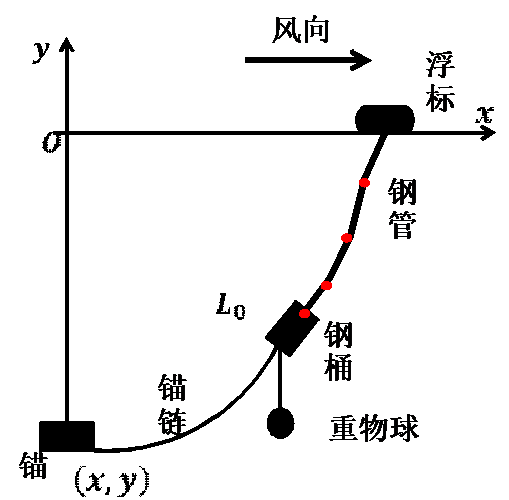
\includegraphics[height=4cm]{images/xiposystem_aixs.jpg}
            \caption{系泊系统整体坐标系}
            \label{fig:系泊系统整体坐标系}
            \end{figure}
            % \textcolor[rgb]{1 0 0}{todo:图片:系泊系统整体坐标系}
            \par
            \textbf{(2)浮标受力分析}
            \par
            浮标系统可简化为底面直径$D$为$2m$、高度$h_0$为$2m$、吃水深度为$h$的圆柱体。当浮标处于平衡状态时,对浮标进行受力分析,浮标会受到重力$G_0$、浮力$F_0$、风力$F_w$、第一根钢管对浮标的拉力$T_1$。浮标的受力情况如图(\ref{fig:浮标受力分析图})所示。
            \begin{figure}[H]
            \centering
            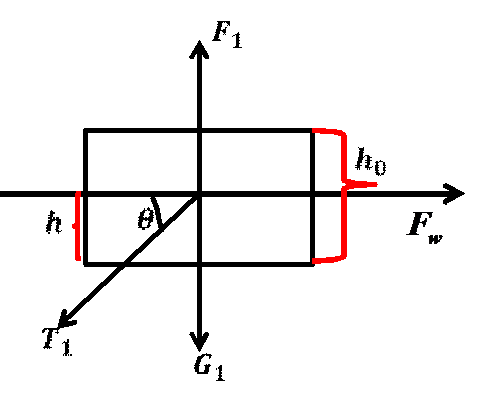
\includegraphics[height=4cm]{images/pipe_force_analysis.jpg}
            \caption{浮标受力分析图}
            \label{fig:浮标受力分析图}
            \end{figure}
            % \textcolor[rgb]{1 0 0}{todo:图片:浮标受力分析图}
            \par
            由浮标质量得出其所受重力$G_0 = m_0g$ ;浮标所受的浮力(当浮标的吃水深度不断变化时排开水体积用积分表示)$F_0 = \rho g\pi (D/2)^2h$ ;由近海风荷载的近似公式可得浮标所受的风力$F_w = 0.625 D(h_0-h)v_w^2$ ;考虑到浮标最终处于静力平衡状态,由静力学平衡方程,有
            \begin{align*}
            & F_0 - G_0 = T_1\sin \theta_1\\
            & F_w = T_1\cos \theta_1
            \end{align*}
            求解上述静力方程,得到第一根钢管对浮标的拉力$T_1$以及与水平面的夹角$\theta_1$
            \begin{align*}
            & T_1 = \sqrt{(F_0-G_0)^2+ F_w^2}\\
            & \theta_1 = \arctan \frac{F_0-G_0}{F_w}
            \end{align*}
            \par
            上述结果中浮标所受的浮力和风力是未知,但均与吃水深度有关,给定一个吃水深度$h$,就会求得一个$\theta_1$,由力学平衡条件得到$T_1$,继而可以计算下面各部分的参数。因此本文稍后会从初始的吃水深度出发,再进行迭代计算。
            \par
            \textbf{(3)钢管受力分析}
            \par
            钢管的受力整体情况如图(\ref{fig:各节钢管所受拉力图})所示,第$i$根钢管的受力分析如图(\ref{fig:单节钢管受力示意图})所示。第$i$根钢管受到重力$G_i$、浮力$F_i$、钢管的上端拉力和下端拉力分别为$T_i$和$T_{i+1},i = 1,2,3,4$。
           \begin{figure}[H]
                \centering
                \begin{subfigure}[b]{0.25\textwidth}
                    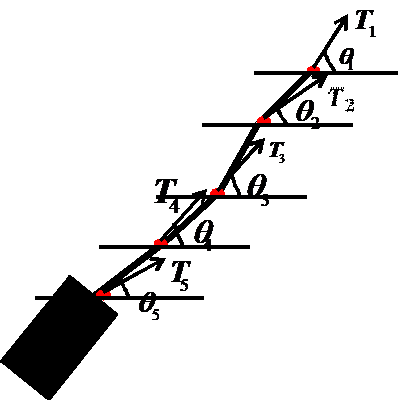
\includegraphics[width=\textwidth]{images/every_steel_force_analysis.jpg}
                    \caption{各节钢管所受拉力图}
                    \label{fig:各节钢管所受拉力图}
                \end{subfigure}
                \qquad
                \begin{subfigure}[b]{0.25\textwidth}
                    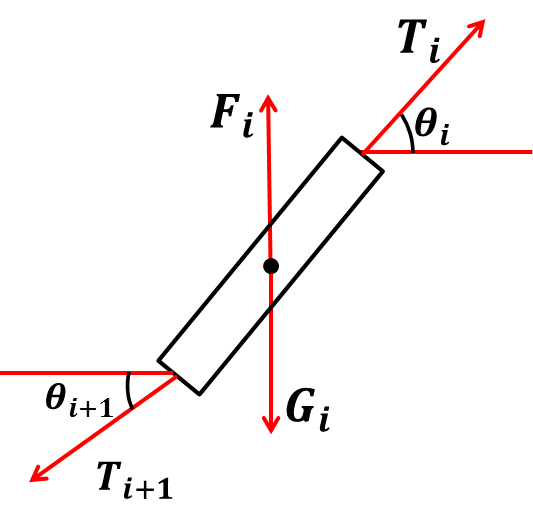
\includegraphics[width=\textwidth]{images/one_steel_force_analysis.jpg}
                    \caption{单节钢管受力示意图}
                    \label{fig:单节钢管受力示意图}
                \end{subfigure}
                % \caption{红旗未旋转前的示意图}
                % \label{fig:红旗未旋转前的示意图}
            \end{figure}
            \par
            根据第$i$根钢管的长度和直径计算钢管的体积,得到钢管所受的浮力大小为
            \begin{align*}
            F_i = \rho g v_i = \rho g S_i l_i
            \end{align*}
            其中:$v_i$为排水体积;$l_i$为钢管的长度,$l_i = 1m$且所有钢管的长度均相同;$D_i$为钢管的直径,且所有钢管的长度均相同,$D_i = 50mm $。且有$S_i = \pi \left( \frac{D_i}{2} \right)^2 $,由物理中的力学得到$\forall i,j\in \{1,2,3,4\}$,均有$F_i = F_j$。
            \par
            钢管处于平衡状态时有静力平衡方程
            \begin{align*}
            & F_i - G_i + T_i\sin \theta_i = T_{i+1}\sin \theta_{i+1}\\
            & T_{i}\cos \theta_i = T_{i+1}\cos \theta_{i+1}
            \end{align*}
            其中,$\theta_i$为第$i$根钢管上端拉力$T_i$与水平方向的夹角;$\theta_{i+1}$为第$i$根钢管下端拉力$T_{i+1}$与水平方向的夹角。求解上述静力方程,就可得到第$i$根钢管所受的拉力及其与水平方向的夹角和相应的坐标$(x_{i+1},y_{i+1})$,注意$(x_{i+1},y_{i+1})$的坐标是由最初的浮标吃水深度$h,x_0$逐步迭代得到的
            \begin{align*}
            & T_{i+1} = \sqrt{(F_{i}-G_i + T_i\sin \theta_i)^2+(T_i\cos \theta_i)^2}\\
            & \theta_{i+1} = \arctan\frac{F_i - G_i + T_i \sin \theta_i}{T_i\cos \theta_i}\\
            & x_{i+1} = x_i - l_i\cos\theta_i\\
            & y_{i+1} = y_i - l_i\sin \theta_i
            \end{align*}
            其中,$l_i$为钢桶的长度,$(x_i,y_i)$为钢桶上端的坐标,$(x_{i+1},y_{i+1})$为钢桶下端的坐标。
            \par
            \textbf{(4)钢桶的受力分析}
            \par
            将钢桶与重物球看成一个整体,分析平衡状态下钢桶整体受到的力,包括重力$G_6$、浮力$F_6$、重物球的重力$G_+$、钢桶上端与下端受到的拉力分别为$T_5$和$T_6$,这里忽略重物球的浮力。钢桶的受力分析如图(\ref{fig:钢桶整体受力示意图})所示。
            \begin{figure}[H]
            \centering
            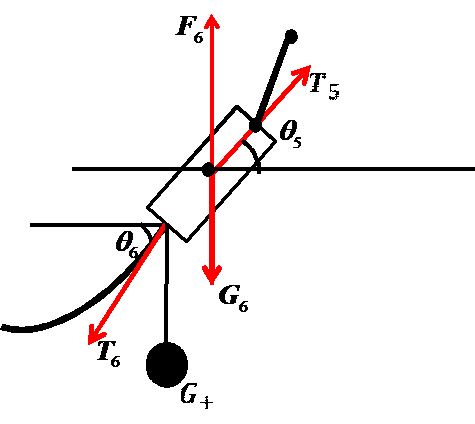
\includegraphics[height=4cm]{images/steel_drums_force_analysis.jpg}
            \caption{钢桶整体受力示意图}
            \label{fig:钢桶整体受力示意图}
            \end{figure}
            \par
            钢桶受到的浮力$F_6$
            \begin{align*}
            F_6 = \rho g l_2 \pi ( {D_2}/{2} ) ^2
            \end{align*}
            其中,$l_2$为钢桶的长,$D_2$为钢桶的横截面直径。然后,钢桶处于平衡状态,由静力平衡方程有
            \begin{align*}
            & (F_6 - G_6 - G_+) +T_5\sin \theta_5 = T_6\sin  \theta_6\\
            & T_5\cos\theta_5 = T_6\cos \theta_6
            \end{align*}
            其中:$\theta_5$为钢桶上端拉力$T_5$与水平方向的夹角,且$\theta_5$与$T_5$通过前面钢管的计算可以得到。因此,求解上述静力平衡方程得到钢桶的下端受到的拉力$T_6$及它与水平方向的夹角$\theta_6$
            \begin{align*}
            & T_6 = \sqrt{(F_6 - G_6 -G_+ +T_5\sin \theta_5)^2+(T_5\cos\theta_5)^2}\\
            & \theta_6 = \arctan \frac{F_6-G_6 - G_++T_5\sin \theta_5}{T_5\cos \theta_5}
            \end{align*}
            \par
            \textbf{(5)锚链的受力分析}
            \par
            在实际的浅海观测网中锚链可能会出现铺底和没有铺底两种情况。设$L_0$为放出锚链总长度,$L$ 为被挂起的锚链长度$L \leqslant L_0$。查阅无档普通链环规格的相关资料可知,II型电焊锚链的半径约为$0.009m$。将锚链看成是长$22.05m$,底面半径为$0.009m$的圆柱体,根据浮力公式计算得到锚链在水下的浮力大小约为$58N$,锚链的重力$G_7 = 1543.5N$,故锚链受到的浮力远远小于重力,因此锚链的浮力对于重力而言可忽略不计。
            由前面的分析可知,我们求得了锚链前端张力$T_6$及张力的水平夹角,同时对锚链的分析可以分为有铺底链和无铺底链两个部分。假设锚链的总长为$L_0$,锚链的单位长度质量为$\bar{m}$,则锚链的水中单位长度重力为$W = \bar{m}g$,则锚链的水下总重力为$G_L = WL$。
            \paragraph{锚链存在铺底链}假设铺底链不存在堆叠现象,即锚链虽然铺底,但它是完全展开的,平铺于海底。以锚的正上方为$y$轴正方向,以海的水平方向为$x$轴,建立直角坐标系,则有铺底链的悬链线受力示意图如图(\ref{fig:有铺底链情况示意图})所示。
            \begin{figure}[H]
            \centering
            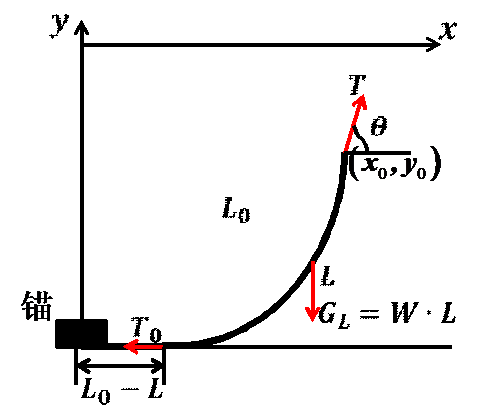
\includegraphics[height=4cm]{images/bottom_chain.jpg}
            \caption{有铺底链情况示意图}
            \label{fig:有铺底链情况示意图}
            \end{figure}
            \par
            上图(\ref{fig:有铺底链情况示意图})中,锚链被提起的长度为$L$,则铺底的锚链长度为$L_0-L$,考虑到有铺底链的受力分析与无铺底链的情况相似,只是坐标可能变化,所以我们直接进行下面的不存在铺底的情况分析。
            \paragraph{锚链不存在铺底}悬链线没有铺底的情况下,即悬链线刚好被完全拉起,其整体受力示意图如图(\ref{fig:没有铺底的悬链线受力示意图})所示。
            \begin{figure}[H]
            \centering
            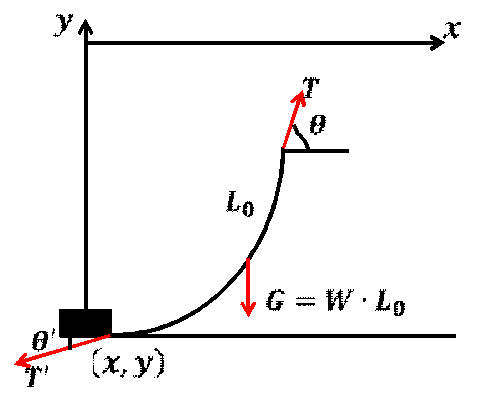
\includegraphics[height=4cm]{images/no_bottom_chain.jpg}
            \caption{没有铺底的悬链线受力示意图}
            \label{fig:没有铺底的悬链线受力示意图}
            \end{figure}
            \par
            假设浮标始终垂直,对锚泊系统我们采用微元法进行分析(单点系泊系统),从锚链中取出一微段$\mathrm{d}s$,微段$\mathrm{d}s$受力情况如图(\ref{fig:微段受力分析示意图})所示。
            \begin{figure}[H]
              \centering
              \begin{varwidth}[t]{\textwidth}
                \vspace{0pt}
                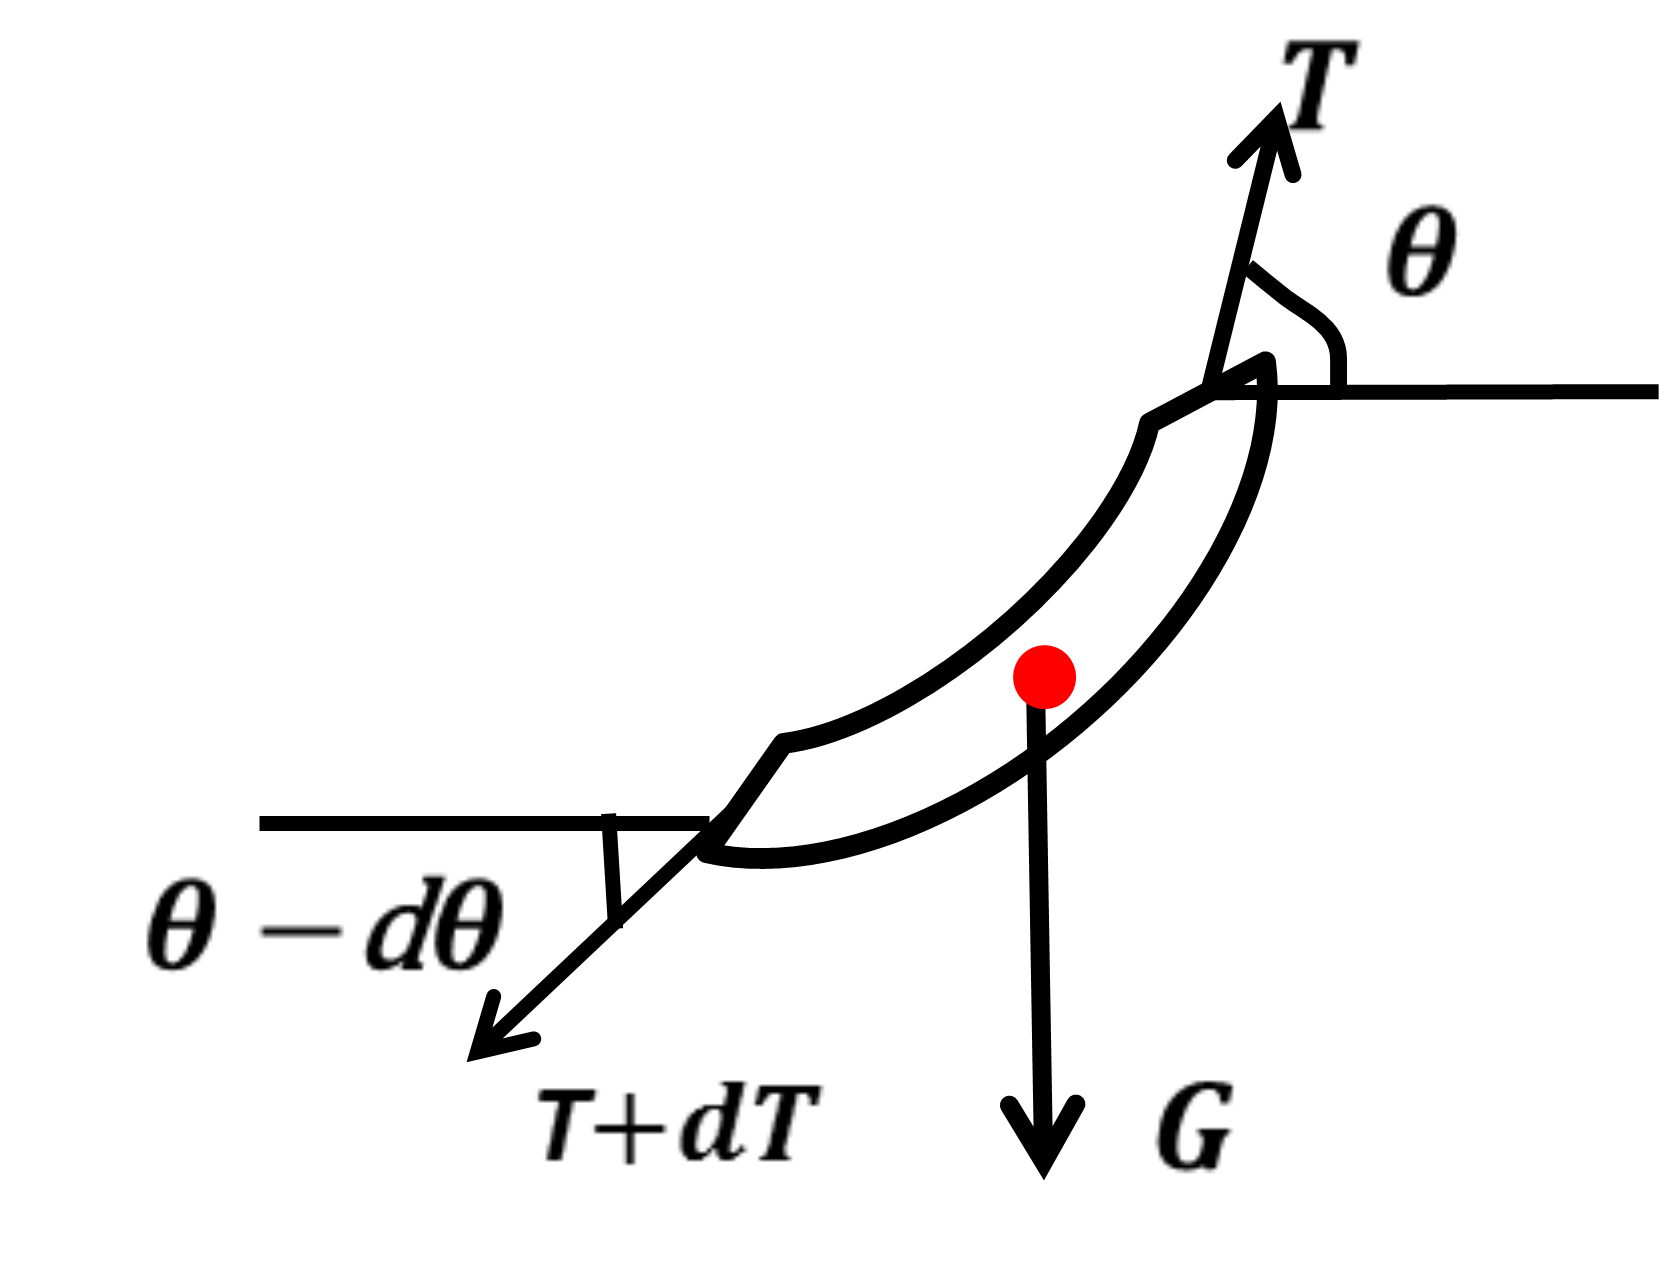
\includegraphics[height=3.5cm]{images/micro_segmehts1.jpg}
              \end{varwidth}
              \qquad
              \begin{varwidth}[t]{\textwidth}
                \vspace{0pt}
                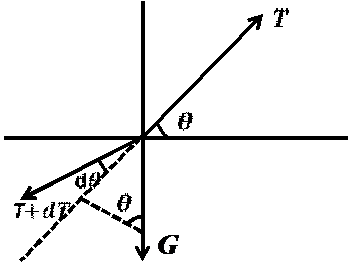
\includegraphics[height=3.5cm]{images/micro_segmehts2.jpg}
              \end{varwidth}
            \caption{微段受力分析示意图}
            \label{fig:微段受力分析示意图}
            \end{figure}
            \par
            锚链某个小段受到的上端与下端张力分别为$T$和$T+\mathrm{d}T$,重力为$G$,$\mathrm{d}T$为拉力的微变量,$\mathrm{d}\theta$为锚链某个小段角度的微变量。根据锚链某个小段的单位长度的重力,可得$\mathrm{d}s$的重力
            \begin{align*}
            G = w\mathrm{d}s
            \end{align*}
            \par
            如图(\ref{fig:微段受力分析示意图})所示,微段$\mathrm{d}s$的静力平衡方程为
            \begin{align}
            \label{微段静力平衡方程}
            & (T+\mathrm{d}T)\sin \mathrm{d}\theta = G\cos\theta\\
            & (T+\mathrm{d}T) \cos \mathrm{d}\theta+G\sin \theta = T\notag
            \end{align}
            将(\ref{微段静力平衡方程})是用泰勒公式展开,忽略二阶无穷小量,当$\mathrm{d}\theta \approx 0$时,有$\cos \mathrm{d}\theta \approx 1,\sin \mathrm{d}\theta \approx \mathrm{d}\theta$,将上式化简得到
            \begin{align}
            \label{微段静力平衡方程1}
            & (T+\mathrm{d}T)\mathrm{d}\theta = G \cos\theta\\
            & (T+\mathrm{d}T) = T - G\sin \theta\notag
            \end{align}
            将上式(\ref{微段静力平衡方程1})化简后的等式转化成递推形式,得到
            \begin{align*}
            & T_{i+1} = T_i -G\sin \theta_i\\
            & \theta_{i+1} = \theta_i - \frac{G\cos\theta_i}{T_i - G\sin \theta_i}
            \end{align*}
            \par
            由此,我们得到$T$和$\theta$的迭代关系式。并且,值得一提的是,该公式在锚链有铺底的情况下同样是适用的。同时,我们注意到坐标变换,有
            \begin{align*}
            \mathrm{d}x = \cos \theta \mathrm{d}s\\
            \mathrm{d}y = \sin \theta \mathrm{d}s
            \end{align*}
            故有
            \begin{align*}
            x_{i+1} = -\cos\theta\mathrm{d}s+x_i\\
            y_{i+1} = -\sin\theta\mathrm{d}s+y_i
            \end{align*}
            在后面的仿真实验中,我们将$L_0$微分成数个$\mathrm{d}s$进行迭代。
        \subsubsection{程序}
            \par
            在上面的受力分析的最后一部分:锚链的受力分析中,我们可以求出锚链每个微元段$\mathrm{d}s$的水平角度$\theta_i$和张力$T_i$,题目要求水深$H$为18$m$,如果锚链有拖尾,当$\theta_i$接近0时,我们就使此部分之后的锚链高度$y_i$不再改变:$y_i = y_{j}(j = i+1,i+2,\dots)$,只改变锚链横坐标即可。并且,我们也得到了系泊系统所有“点”的郑横纵坐标。
            \par
            经过上面的分析,我们发现:在其它条件给定的情况下(风速、水密度、链型、链长和重物球),每给定一个浮漂吃水深度$h$,我们就可以有一个系泊系统的整体深度,换句话说,我们将其它条件视(风速、水密度、链型、链长和重物球)为参数$\theta$,吃水深度视为自变量$x$,系泊系统整体深度视为因变量$y$,则我们找到了二者之间的函数关系$y = f(x;\theta)$。题目中给定海水深度为$18m$,也就是说,我们只要求解$y=18$时的自变量值$x$(即吃水深度$h$)即可。当$h$求解出来之后,整个系泊系统的各点的坐标、角度以及张力也就有了。
            \par
            下面,我们先给出系泊系统各个量之间的关系。为了简单,我们记吃水深度$h\triangleq  -y_0$,浮漂的横坐标为$x_0$,各个量之间的关系函数如下,编写为For2D.m
            \begin{lstlisting}[language = Matlab]
            function [y, x, theta, T, stat] = For2D(y0, x0, v_wind, m_qiu, I, L, xitong_figure)
            % 此函数用于给定x0和y0后求解系泊系统的状态曲线
            %
            %%%%输入%%%%
            % y0:浮标纵坐标,|y0|=h。其中,h为吃水深度。
            % x0:浮标横坐标。
            % v_wind:风速。
            % m_qiu:重物球质量。
            % I:锚链型号。1、2、3、4、5
            % L:锚链长度。
            % outputfigure:是否输出系统图像。logistic
            %
            %%%%输出%%%%
            % y:系泊系统纵坐标。向量
            % x:系泊系统横坐标。
            % theta:系泊系统角度。
            % T:系泊系统拉力。
            % stat:要求的系泊系统参数,包括:吃水深度h、横坐标x0、游动区域S、钢桶竖直夹角alpha1、锚链底端水平夹角alpha2、风速v_wind、重物球质量m、系统状态yxthetaT。stats
            %%%%正文%%%%
            %确定锚链
            switch I
                case 1
                   II = 78/1000;%锚链每节长度 m
                   m_II = 3.2;%单位长度的质量 kg/m
                case 2
                   II = 105/1000;%锚链每节长度 m
                   m_II = 7;%单位长度的质量 kg/m
                case 3
                   II = 120/1000;
                   m_II = 12.5;%单位长度的质量 kg/m
                case 4
                    II = 150/1000;
                    m_II = 19.5;%单位长度的质量 kg/m
                case 5
                    II = 180/1000;
                    m_II = 28.12;%单位长度的质量 kg/m
            end
            n = round(L/II);
            ind = n+5+1;
            y(1) = y0;
            x(1) = x0;
            h = abs(y(1));%浮标吃水深度
            %浮标受力
            rho = 1.025*10^3;%海水的密度  kg/m^3
            g = 9.8;%重力加速度 N/kg
            D = 2;%圆柱浮标地面直径 m
            h0 = 2;%圆柱浮标高度 m
            m0= 1000;%浮标质量 kg
            F0 = rho*g*pi*(D/2)^2*h;%浮标浮力
            G0 = m0*g;%浮标重力
            %v_wind = 12;%风速 m/s
            S_wind = D*(h0-h);%风受力面积
            F_wind = 0.625*S_wind*v_wind^2;%风力
            theta1 = atan((F0-G0)/F_wind);%钢管1的水平夹角
            T1 = sqrt((F0-G0)^2+(F_wind)^2);%钢管1的张力
            T(1) = T1; theta(1) = theta1;
            %钢管受力分析
            for i = 1:4
                m(i) = 10;%钢管质量 kg
                G(i) = m(i)*g;%钢管重力
                l(i) = 1;%钢管长度 m
                d(i) = 50/1000;%钢管直径 m
                F(i) = rho*g*pi*(d(i)/2)^2*l(i);%钢管浮力

                T(i+1) = (  (F(i)-G(i)+T(i)*sin(theta(i)))^2  +...
                    (T(i)*cos(theta(i)))^2    )^(1/2);
                theta(i+1) = atan(  (  (F(i)-G(i)+T(i)*sin(theta(i)))/...
                    (T(i)*cos(theta(i)) ))   );

                %钢管i的坐标(xi,yi)
                y(i+1) = y(i) - l(i)*sin(theta(i));
                x(i+1) = x(i) - l(i)*cos(theta(i));
            end
            %钢桶受力分析
            m_tong = 100;%钢桶的质量 kg
            G_tong = m_tong*g;%钢桶重力
            % m_qiu = 1200;%重物球质量 kg
            G_qiu = m_qiu*g;%重物球重力
            l_tong = 1;%钢桶长 m
            D_tong = 30/100;%钢桶底长
            F_tong = rho*g*pi*(D_tong/2)^2*l_tong;%钢桶浮力
            T_tong = ( (F_tong-G_tong-G_qiu+T(5)*sin(theta(5)))^2 + ...
                            (T(5)*cos(theta(5)))^2)^(1/2);
            theta_tong = atan( ((F_tong-G_tong-G_qiu+T(5)*sin(theta(5)))...
                                  /(T(5)*cos(theta(5)))) );
            T(6) = T_tong;
            theta(6) = theta_tong;
            y(6) = y(5) - l_tong*sin(theta(5));
            x(6) = x(5) - l_tong*cos(theta(5));
            %锚链线分析
            G_mao = II*m_II*g;%单位长度重量
            L_tuo = 0;%锚链拖尾长度
            for i = 6 : 6+n-1
                if  theta(i) - 0 > 0.001
                    T(i+1) = T(i) - G_mao*sin(theta(i));
                    theta(i+1) = theta(i) - (G_mao*cos(theta(i)))/(T(i)-G_mao*sin(theta(i)));
                    y(i+1) = y(i) - sin(theta(i))*II;
                    x(i+1) = x(i) - cos(theta(i))*II;
                else
                    T(i+1) = 0;
                    theta(i+1) = 0;
                    y(i+1) = y(i);
                    x(i+1) = x(i) - II;
                    L_tuo = L_tuo+II;
                end
            end
            \end{lstlisting}
            \par
            上面给出了系泊系统各个量之间的关系函数For2D,下面,我们就求解系泊系统深度$y(end)=18m$时的吃水深度$h$。这里,我们提供三种方法:
            \par
            (1).离散枚举法,将$h$从$[0,2]$遍历离散取值,选取$y(end)$最接近$18$的$h$,函数为bestpoint.m,如下
            \begin{lstlisting}[language = Matlab]
            function [besty0, bestx0] = bestpoint(H, N, x0, v_wind, m_qiu, I, L, y0_yn_figure)
            %此函数用离散枚举法求最优吃水深度h
            %
            y0 = linspace(0, -2, N);
            %注:y0是有取值范围的,y0不可以从0开始取值,否则会发生yn>0的情况。
            %修正y0
            rho = 1.025*10^3;%海水的密度  kg/m^3
            D = 2;%圆柱浮标地面直径 m
            m0= 1000;%浮标质量 kg
            y0_min = -(m0+m_qiu)/(rho*pi*(D/2)^2);
            y0 = linspace(y0_min, -2, N);
            yn = zeros(size(y0));
            xn = zeros(size(y0));
            xitong_figure = 0;
            for i = 1:length(y0)
                [y, x, theta, ~] = For2D(y0(i), x0, v_wind, m_qiu, I, L, xitong_figure);
                yn(i) =  y(end);
                xn(i) =  x(end);
                thetan(i) = theta(end - 1);
            end

            [~, ind1] = min(abs(yn - (-H)));
            besty0 = y0(ind1);
            bestx0 = x0 - xn(ind1);
            \end{lstlisting}
            \par
            (2)迭代算法求最优吃水深度。这种方法是有方向的调整吃水深度,是系泊系统水深和$18m$接近,函数为bestpoint2.m,如下
            \begin{lstlisting}[language = Matlab]
            function [besty0, bestx0, bestyn] = bestpoint2(y0, x0, H, eta, maxt, eps, v_wind, m_qiu, I, L)
            %此函数用迭代算法求最优吃水深度h
            %%%%正文%%%%
            xitong_figure = 0;
            t = 0;
            while t < maxt
                [~, ~, ~, ~, stat] = For2D(y0, x0, v_wind, m_qiu, I, L, xitong_figure);
                yn = stat.yn;
                xn = stat.xn;
                delta_yn = yn - (-H);
                if abs(delta_yn) < eps
                    disp('yn满足精度,终止')
                    break;
                else
                    y1 = y0;
                    y0 = y0 - eta*delta_yn;%更新y0
                    %如果y0不在范围内
                    if y0 < -2 | y0 > 0
                        eta1 = 0.5*eta;
                        y0 = y1 - eta1*delta_yn;
                    end
                end
                t = t+1;
                if t == maxt
                    disp('达到最大迭代次数,终止')
                end
            end
            %%%%构建输出%%%%
            disp(['迭代次数:', num2str(t)])
            besty0 = y0;
            bestyn = yn;
            bestx0 = x0 - xn;
            \end{lstlisting}
            \par
            (3)用fzero法求最优吃水深度。其实,对于这个函数问题,我们可以使用MATLAB自带的函数命令fzeros来求解,求解程序如下
            \begin{lstlisting}[language = Matlab]
            function [besty0, bestx0] = bestpoint3(H, x0, v_wind, m_qiu, I, L, xitong_figure)
            %此函数用fzero法求最优吃水深度h
            %
            fun = @(y0)bestpoint3fun(y0, H, x0, v_wind, m_qiu, I, L, xitong_figure);
            y0 = -0.3; % initial point
            besty0 = fzero(fun, y0);
            [~, x, ~, ~, ~] = For2D(besty0, x0, v_wind, m_qiu, I, L, xitong_figure);
            bestx0 = x0 - x(end);
            end

            function f = bestpoint3fun(y0, H, x0, v_wind, m_qiu, I, L, xitong_figure)
            %此函数用于构建fzero函数的输入,以求解yn = -H。
            %
            [y, ~, ~, ~, ~] = For2D(y0, x0, v_wind, m_qiu, I, L, xitong_figure);
            yn = y(end);
            f = yn - (-H);
            end
            \end{lstlisting}
            \par
            下面,我们给出求解各风速下系泊系统的状态的程序
            \begin{lstlisting}[language = Matlab]
            %% 利用离散枚举法计算bestx0, besty0情况下的系统信息及系统图形
            %风速为12时的系统情况
            H = 18; N = 1000; x0 = 20; v_wind = 12;
            m_qiu = 1200; I = 2; L = 22.05;
            y0_yn_figure = 1; xitong_figure = 1;
            [besty0, bestx0] = bestpoint(H, N, x0, v_wind, m_qiu, I, L, y0_yn_figure);
            y0 = besty0;
            x0 = bestx0;
            [y1, x1, theta1, T1, stat1] = For2D(y0, x0, v_wind, m_qiu, I, L, xitong_figure);
            \end{lstlisting}
        \subsubsection{结果}
            \par
            风速$v_w=12m/s$时锚链末端$y_n$和水平夹角随吃水深度$h$的变化曲线如图(\ref{风速12时锚链末端及水平夹角随吃水深度h的变化曲线})所示,我们只要选取末端$y_n = 18$时的吃水深度即可,称此吃水深度为最优吃水深度。
            \begin{figure}[H]
                \centering
                \begin{subfigure}[b]{0.4\textwidth}
                    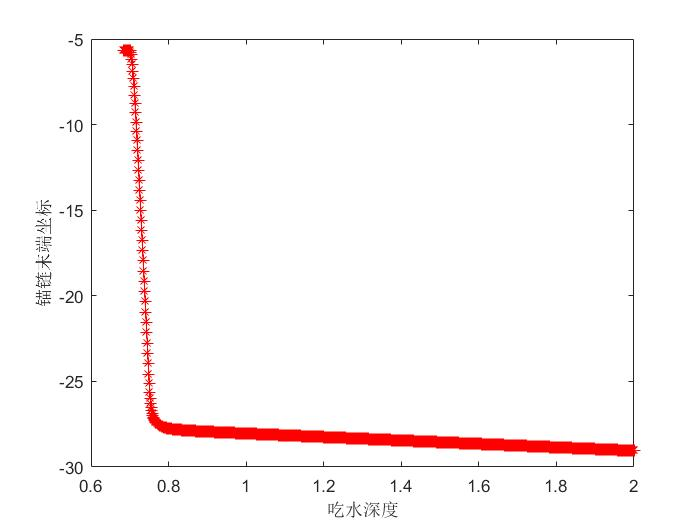
\includegraphics[width=\textwidth]{images/v_wind_12_yn_h.jpg}
                    % \caption{}
                \end{subfigure}
                \begin{subfigure}[b]{0.4\textwidth}
                    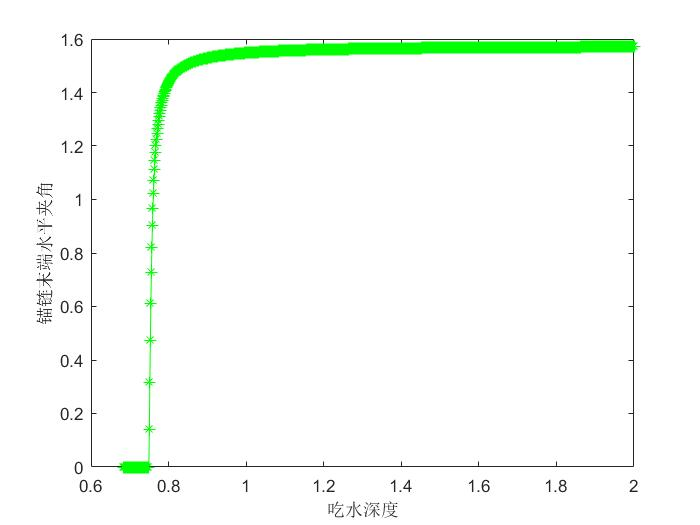
\includegraphics[width=\textwidth]{images/v_wind_12_alpha_h.jpg}
                    % \caption{}
                \end{subfigure}
                \caption{风速12时锚链末端及水平夹角随吃水深度h的变化曲线}
                \label{风速12时锚链末端及水平夹角随吃水深度h的变化曲线}
            \end{figure}
            在最优吃水深度下,系泊系统的系统曲线如图(\ref{风速12、吃水深度0.73461时的系泊系统})所示。最优的$h$为$0.734 $,$(x_1,y_1)=(14.416,-0.734)$,浮标的游动面积为628.343$m^2$ 。
            \begin{figure}[H]
                \centering
                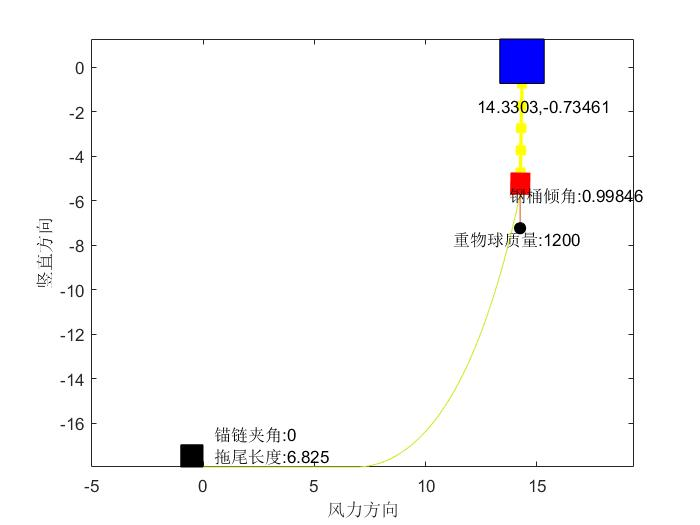
\includegraphics[width=8cm]{images/v_wind_12_h_xitong.jpg}
                \caption{风速12、吃水深度0.73461时的系泊系统}
                \label{风速12、吃水深度0.73461时的系泊系统}
            \end{figure}
            \par
            风速$v_w=24m/s$时锚链末端$y_n$和水平夹角随吃水深度$h$的变化曲线如图(\ref{风速24时锚链末端及水平夹角随吃水深度h的变化曲线})所示。
            \begin{figure}[H]
                \centering
                \begin{subfigure}[b]{0.4\textwidth}
                    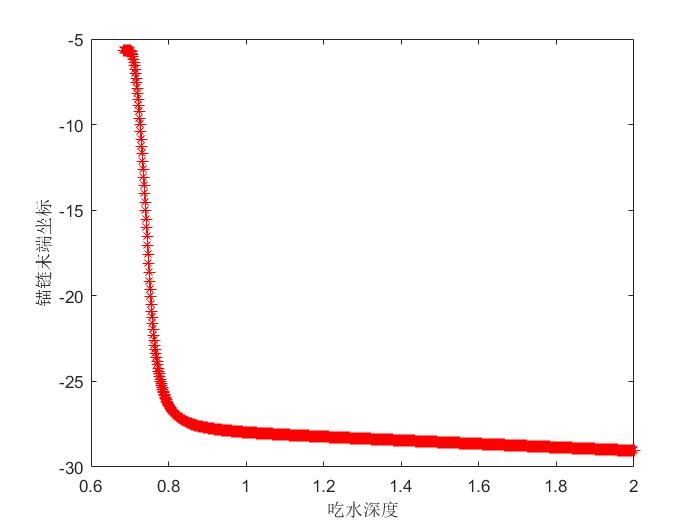
\includegraphics[width=\textwidth]{images/v_wind_24_yn_h.jpg}
                    % \caption{}
                \end{subfigure}
                \begin{subfigure}[b]{0.4\textwidth}
                    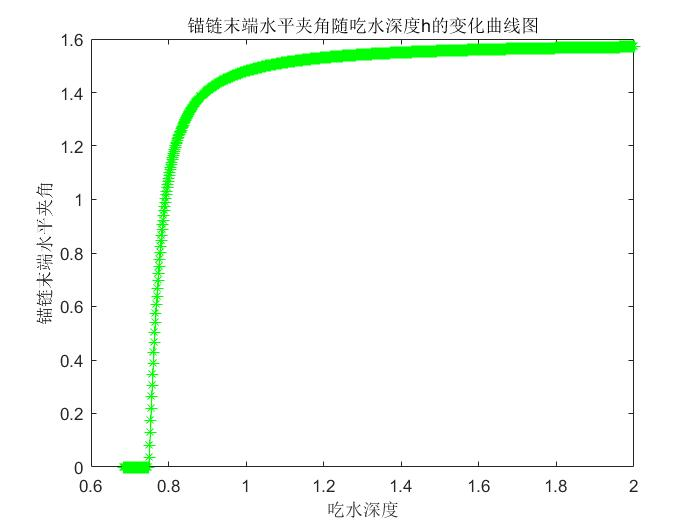
\includegraphics[width=\textwidth]{images/v_wind_24_alpha_h.jpg}
                    % \caption{}
                \end{subfigure}
                \caption{风速24时锚链末端及水平夹角随吃水深度h的变化曲线}
                \label{风速24时锚链末端及水平夹角随吃水深度h的变化曲线}
            \end{figure}
            在最优吃水深度下,风速$v_w=24m/s$时系泊系统的系统曲线如图(\ref{风速24、吃水深度0.74911时的系泊系统})所示。
            \begin{figure}[H]
                \centering
                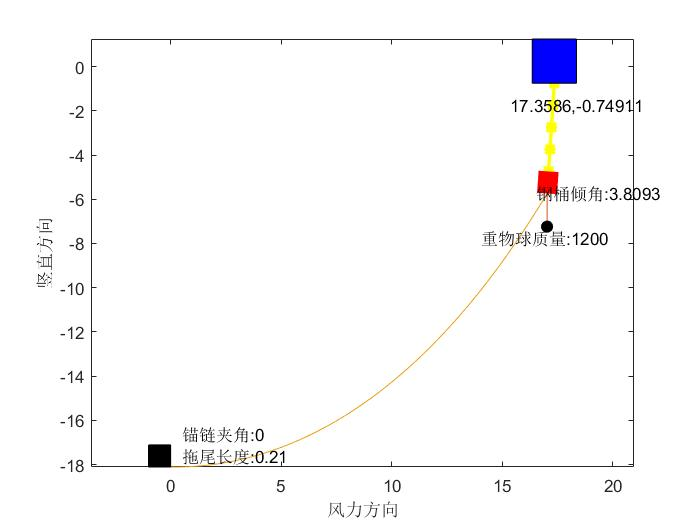
\includegraphics[width=8cm]{images/v_wind_24_h_xitong.jpg}
                \caption{风速24、吃水深度0.74911时的系泊系统}
                \label{风速24、吃水深度0.74911时的系泊系统}
            \end{figure}


    \subsection{问题二的分析与求解}
        \subsubsection{问题的分析}
            \par
            问题要求我们在问题1的假设下,在风速$v=36m/s$,重新计算各指标。并调节重物球的质量,使得钢桶的倾斜角度不超过$5^\circ$,锚链末端与锚的链接处的切线方向与海床的夹角不超过$16^\circ$。
            \par
            题目的意思是:在风速$v=36m/s$时系泊系统整体状态的时候,由于风力太大,使得浮漂整体被拉起(钢桶的倾斜角度和锚链末端与锚的链接处的切线方向与海床的夹角就变得很大),吃水深度很深。因此,我们要增加重物球的质量,使链拉的没有那么“直”。我们可以考虑建立优化模型,这个优化模型的目标其实在题目中已经给出了,“系泊系统的设计问题就是确定锚链的型号、长度和重物球的质量,使得浮标的吃水深度和游动区域及钢桶的倾斜角度尽可能小。”,我们由此来设计优化模型的目标及约束条件。并且,注意到这个系泊系统的设计是多目标的(这几个目标之间相互矛盾),为此,我们采用IENSGA\rom{2}算法进行求解。

        \subsubsection{模型的建立与求解}
            \par
            问题二的前半部分只是重新给出了一个风速,所以与第一问的思路相同,这里只给出一个结果。在最优吃水深度下,风速$v_w=36m/s$时系泊系统的系统曲线如图(\ref{风速36、吃水深度0.7702时的系泊系统})所示。
            \begin{figure}[H]
                \centering
                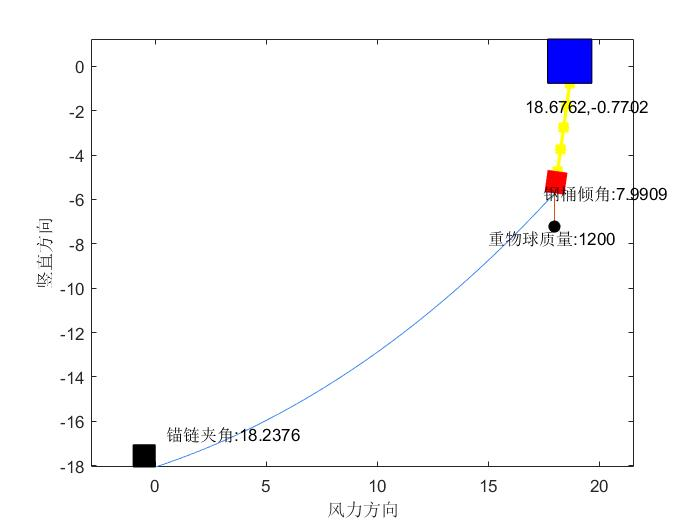
\includegraphics[width=8cm]{images/v_wind_36_h_xitong.jpg}
                \caption{风速36、吃水深度0.7702时的系泊系统}
                \label{风速36、吃水深度0.7702时的系泊系统}
            \end{figure}
            \par
            风速$v=36m/s$时系泊系统的最优浮漂位置$(x_0,y_0) = (18.6505,-0.7704)$,浮漂吃水深度为$h = 0.7704$ ,第一根到第四根钢管和钢桶与竖直方向的夹角弧度数分别为1.4344、1.4336、1.4329、1.4322、1.4314。这时,我们发现系泊系统的角度非常大,这是相当不稳定的。为此,要调节重物球的质量使系泊系统的各夹角变小。我们定义$m_+$为重物球的质量,$\alpha_1$为钢桶与竖直方向的夹角,它与锚链与水平方向的夹角$\theta_5$互余,即$\alpha_1 = 90^\circ - \theta_5$。$\alpha_2$为锚链末端与水平方向的夹角。通过不断的调整$m_+$,使得$\alpha_5$不超过$5^\circ$,$\alpha_2$不超过$16^\circ$。我们可以建立一个优化问题。
            \par
            \begin{enumerate}
            \item 首先,我们设定优化模型的优化变量为重物球质量$m_+$。
            \item 然后,我们设定优化的目标是:吃水深度$h$最小、$\alpha_1$夹角最小、游动面积最小。但3者不可能同时达到最小,故而有下面的多目标优化的处理。
            \item 最后,我们设置优化的约束条件:要求$\alpha_1$在$[0,5]$范围内,$\alpha_2$在$[0,16]$范围内进行取值。但是,这里我们重物球的质量$m_+$的取值范围,为此,我们要先分析一下$m_+$。
            \end{enumerate}
            \par
            我们先来分析一下$m_+$。分析一下下面的关系:1.$m$与$y_0$的关系;2.$m$与$x_0$的关系;3.$m$与$\alpha_1$的关系;4.$m$与$\alpha_2$的关系;并且注意到,我们要求解使$\alpha_1,\alpha_2$满足要求的最小的$m_+$,即$m_+$的下限。然后,我们根据$m$与$y_0$的关系来求解$m_+$的上限。
            \paragraph{$m$与$y_0$的关系}浮标的吃水深度$h$随重物球质量$m_+$的变化趋势如图(\ref{fig:吃水深度h随重物球质量变化曲线})所示。从图中可以看出,浮标的吃水深度$h$与重物球质量$m_+$大约成正相关的线性关系。当重物球的质量为$5200kg$左右时,浮标的吃水深度达到最大$h=2m$,此后再增加重物球的质量,浮标的吃水深度不再改变。
            \paragraph{$m$与$x_0$的关系}浮标横坐标$x_0$(游动范围$S$)随重物球质量$m_+$的变化趋势如图(\ref{fig:浮漂横坐标随重物球质量变化曲线})所示从图中可以看出,浮标横坐标$x_0$与重物球质量$m_+$成反比例关系,重物球质量越大,浮标横坐标越小,游动范围越小。
            \paragraph{$m$与$\alpha_1$的关系}钢桶竖直夹角$\alpha_1$随重物球质量$m_+$的变化趋势如图(\ref{fig:钢桶竖直夹角随重物球质量变化曲线})所示从图中可以看出,钢桶竖直夹角$\alpha_1$与重物球质量$m_+$成反比例关系,重物球质量越大,钢桶竖直夹角$\alpha_1$越小。当重物球质量达到 $5200kg $时,钢桶竖直方向夹角达到$ 0 $度。与此同时,我们可以找到钢桶竖直夹角$\alpha_1=\frac{5}{90}\frac{\pi}{2}$时的重物球质量$m_1 = 1808kg$。也就是说,要使钢桶竖直夹角$\alpha_1 <5^\circ$,重物球质量要大于$1808kg $。
            \paragraph{$m$与$\alpha_2$的关系}锚链底端水平夹角$\alpha_2$随重物球质量$m_+$的变化趋势如图(\ref{fig:锚链底端水平夹角随重物球质量变化曲线})所示从图中可以看出,锚链底端水平夹角$\alpha_2$与重物球质量$m_+$成反比例关系,重物球质量越大,锚链底端水平夹角$\alpha_2$越小。当重物球质量达到 $5200kg $时,锚链底端水平夹角达到$0^\circ$。与此同时,我们可以找到锚链底端水平夹角$\alpha_2=\frac{16}{90}\frac{\pi}{2}$时的重物球质量$m_2 = 1202kg$。也就是说,要使锚链底端水平夹角$\alpha_2 <16^\circ$,重物球质量要大于$1202kg $。
            \begin{figure}[H]
                \centering
                \begin{subfigure}[b]{0.4\textwidth}
                    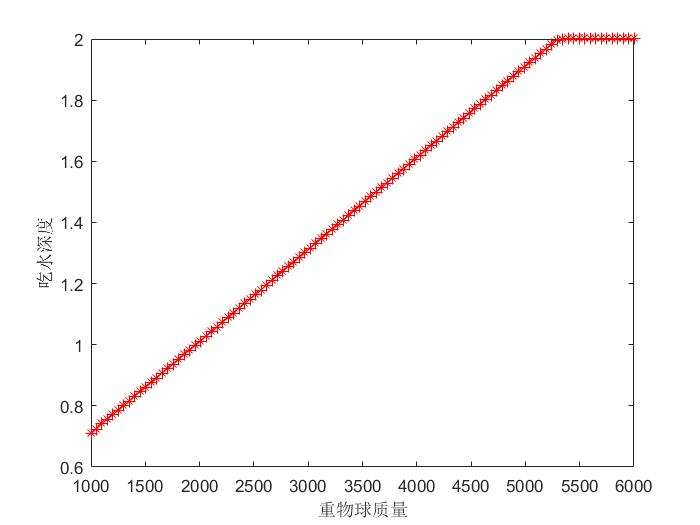
\includegraphics[width=\textwidth]{images/h_m+.jpg}
                    \caption{}
                    \label{fig:吃水深度h随重物球质量变化曲线}
                \end{subfigure}
                \begin{subfigure}[b]{0.4\textwidth}
                    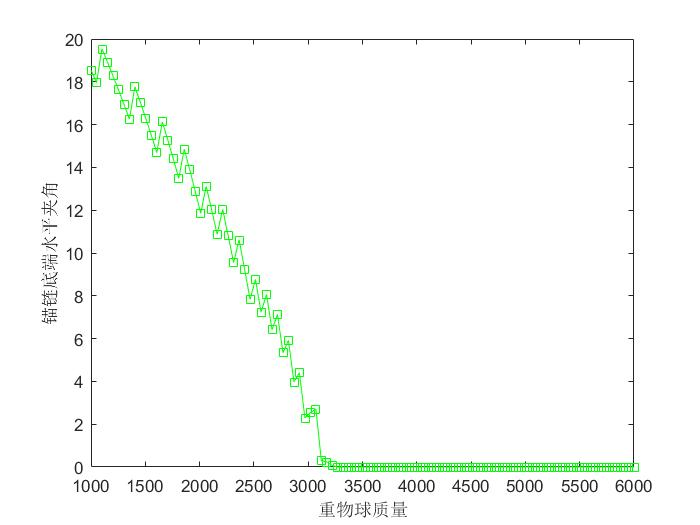
\includegraphics[width=\textwidth]{images/alpha2_m+.jpg}
                    \caption{}
                    \label{fig:锚链底端水平夹角随重物球质量变化曲线}
                \end{subfigure}
                \centering
                \begin{subfigure}[b]{0.4\textwidth}
                    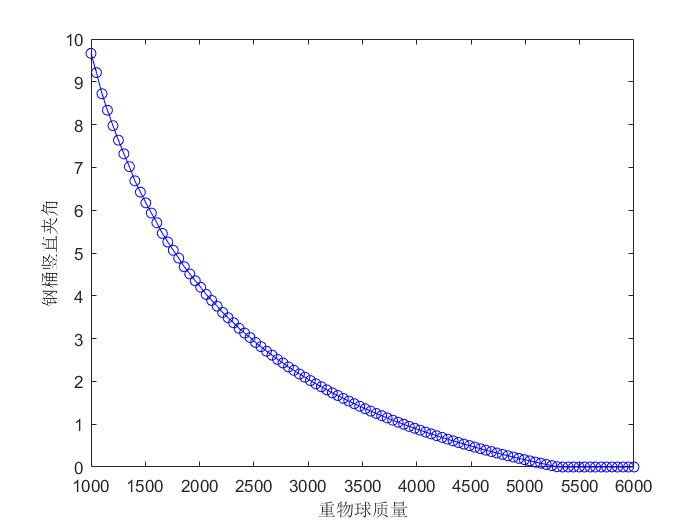
\includegraphics[width=\textwidth]{images/alpha1_m+.jpg}
                    \caption{}
                    \label{fig:钢桶竖直夹角随重物球质量变化曲线}
                \end{subfigure}
                \begin{subfigure}[b]{0.4\textwidth}
                    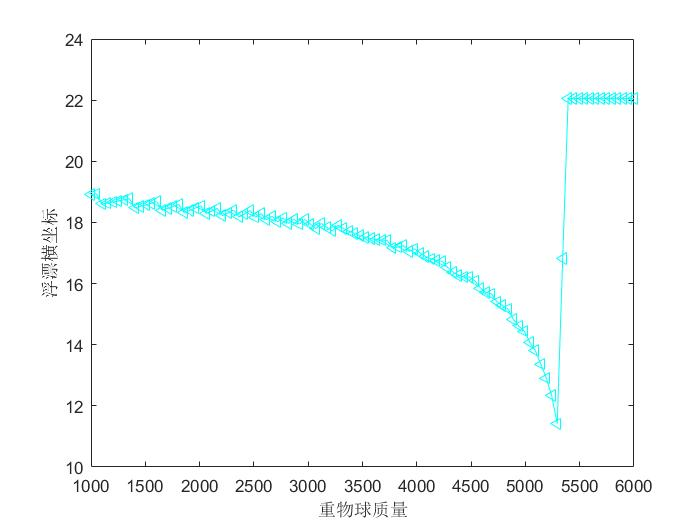
\includegraphics[width=\textwidth]{images/x0_m+.jpg}
                    \caption{}
                    \label{fig:浮漂横坐标随重物球质量变化曲线}
                \end{subfigure}
                \caption{重物球质量与各变量间的关系图}
                \label{重物球质量与各变量间的关系图}
            \end{figure}
            \par
            经过上面对重物球质量$m_+$的分析,如果单从第二问来看,满足要求的重物球质量范围为$[1808,5200]$,此范围内的重物球都可以使钢桶竖直夹角$\alpha_1 <5^\circ$锚链底端水平夹角$\alpha_2 <16^\circ$(最终获得的重物球质量$m_+$的取值范围为$ m_1= 1757.6, m_2=1656.6, m_3=5393.9$,即$1757.6<m_+<5393.9$。)。下面,我们来建立优化模型,求解合适的重物球质量$m_+$。我们建立优化模型,求最优$m_+$,使得$h$、$\alpha_1$和面积$\pi x_0^2$最小,有
            \begin{align}
            \label{系泊系统优化模型1}
            & \min_{m_+} \ \{h,\alpha_1,\pi x_0^2\}\\
            & s.t.\left\{
            \begin{aligned}
            & 0 < \alpha_1 \leqslant \frac{5}{90}\frac{\pi}{2}\\
            & 0 < \alpha_2 \leqslant \frac{16}{90}\frac{\pi}{2}\\
            & \max\{m_1,m_2\} < m_+ < 6000
            \end{aligned}
            \right.\notag
            \end{align}
            \par
            这里有一点要说明的是,上面模型中的第3个约束就是由前两个约束变化而来的,所以在实际编程中,只需要考虑第三个约束即可。上面建立的优化模型有三个目标,并不容易处理。根据前面对$m_+$的分析,我们可以发现:$m_+$与$h$成正比关系,而与$\alpha_1,\alpha_2$以及游动范围$\pi x_0^2$成反比例关系。
            为此,我们将其规整为两目标优化模型,将目标$\alpha_1$和$\pi x_0^2$合并,并设置目标权重为$c$,有
            \begin{align}
            \label{系泊系统优化模型2}
            & \min_{m_+}\ \left\{
            \begin{aligned}
            & h\\
            & \alpha_1+c\pi x_0^2
            \end{aligned}
            \right.\\
            & s.t.\left\{
            \begin{aligned}
            & 0 < \alpha_1 \leqslant \frac{5}{90}\frac{\pi}{2}\\
            & 0 < \alpha_2 \leqslant \frac{16}{90}\frac{\pi}{2}\\
            & \max\{m_1,m_2\} < m_+ < 6000
            \end{aligned}
            \right.\notag
            \end{align}
            其中,$c$为目标权重系数(外来参数);为了方便计算,上述约束条件中的$\alpha_1$与$\alpha_2$均要转换成弧度;同时,模型中的角度及坐标还要满足系泊系统静态平衡时的方程。下面,来简单分析一下上述优化问题。这是一个多目标优化问题,给定$m_+$后,并不能使$h,\alpha_1+c\pi x_0^2$同时达到最小。要解决这样的多目标优化问题,我们可以采用IENSGA\rom{2}算法的思想对其进行求解。Pareto最优解如图(\ref{系泊系统多目标规划的Pareto前端})所示
            \begin{figure}
                \centering
                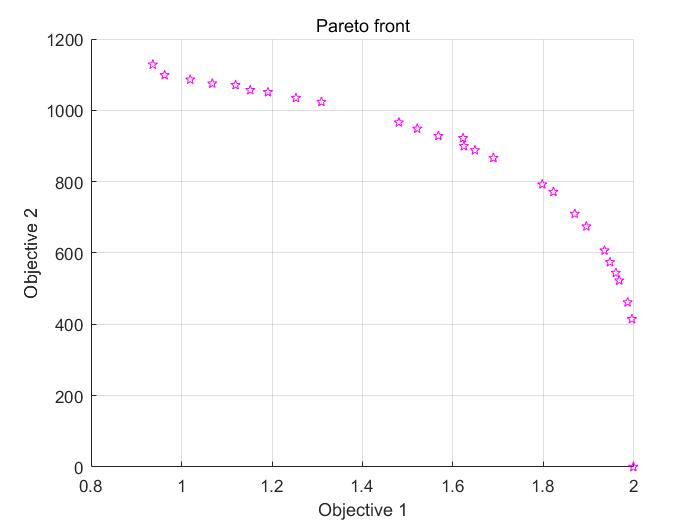
\includegraphics[width = 6cm]{images/pareto_qiandan.jpg}
                \caption{系泊系统多目标规划的Pareto前端}
                \label{系泊系统多目标规划的Pareto前端}
            \end{figure}
            \par
            模型(\ref{系泊系统优化模型1})可以变为2个目标,也可以变为1个目标。在第二问中,我们将其规整为2个目标并用IENSGA\rom{2}求解。但是在第三问中,题目要求我们在多个方案中挑选最优方案,所以我们要用唯一的目标来衡量各个方案,而不是Pareto最优解,因此,在第三问当中,我们把模型(\ref{系泊系统优化模型1})规整为1个目标,用GA算法及fmincon进行求解。

        \subsubsection{程序}
            \par
            这里,我们先给出模型(\ref{系泊系统优化模型2})的目标函数multi$\_$GA$\_$m的程序
            \begin{lstlisting}[language = Matlab]
            function f = multi_GA_m(m_qiu)
            %此函数是IENSGAii的目标函数。
            %
            %解为m_qiu
            %目标1:吃水深度最小
            %目标2:游动区域和钢桶夹角最小
            %
            %正文
            %定参
            v_wind = 36;
            %超参
            c = 10;
            H = 18;
            N = 500;
            x0 = 20;
            I = 2;
            L = 22.05;
            y0_yn_figure = 0;
            xitong_figure = 0;

            [besty0, bestx0] = bestpoint(H, N, x0, v_wind, m_qiu, I, L, y0_yn_figure);
            [~, ~, ~, ~, stat] = For2D(besty0, bestx0, v_wind, m_qiu, I, L, xitong_figure);
            alpha1 = stat.alpha1;

            f(1) = abs(besty0);
            f(2) = pi*bestx0^2 + c*alpha1;
            end
            \end{lstlisting}
            然后,我们给出第二问的具体求解程序,如下
            \begin{lstlisting}[language = Matlab]
            %% 绘制m_qiu和y0 、x0 、alpha1、alpha2之间的关系图
            clc
            clear
            %定参
            v_wind = 36;
            %超参
            H = 18;
            N = 500;
            x0 = 20;
            I = 2;
            L = 22.05;
            y0_yn_figure = 0;
            xitong_figure = 0;
            %正文
            m_qiu = linspace(1000, 6000, 100);
            besty0 = zeros(size(m_qiu));
            bestx0 = zeros(size(m_qiu));
            alpha1 = zeros(size(m_qiu));
            alpha2 = zeros(size(m_qiu));
            for i = 1:length(m_qiu)
                [besty0(i), bestx0(i)] = bestpoint(H, N, x0, v_wind, m_qiu(i), I, L, y0_yn_figure);
                y0 = besty0(i);
                x0 = bestx0(i);
                [~, ~, ~, ~, stat] = For2D(y0, x0, v_wind, m_qiu(i), I, L, xitong_figure);
                alpha1(i) = stat.alpha1;
                alpha2(i) = stat.alpha2;
            end
            %绘图
            figure(1)
            plot(m_qiu, abs(besty0), 'r*-')
            xlabel('重物球质量')
            ylabel('吃水深度')
            title('吃水深度h随重物球质量变化曲线')
            figure(2)
            plot(m_qiu, bestx0, 'c<-')
            xlabel('重物球质量')
            ylabel('浮漂横坐标')
            title('浮漂横坐标随重物球质量变化曲线')
            figure(3)
            plot(m_qiu, alpha1, 'bo-')
            xlabel('重物球质量')
            ylabel('钢桶竖直夹角')
            title('钢桶竖直夹角随重物球质量变化曲线')
            figure(4)
            plot(m_qiu, alpha2, 'gs-')
            xlabel('重物球质量')
            ylabel('锚链底端水平夹角')
            title('锚链底端水平夹角随重物球质量变化曲线')
            %注:最好插值or拟合一下。

            %% 确定m_qiu的取值范围
            %钢桶的倾斜角度不超过5度,锚链在锚点与海床的夹角不超过16度
            alpha1_max = 5;
            alpha2_max = 16;

            [~, ind1] = min(abs(alpha1 - alpha1_max));
            m1 = m_qiu(ind1);
            [~, ind2] = min(abs(alpha2 - alpha2_max));
            m2 = m_qiu(ind2);
            %浮漂完全没入水中,h = 2。
            ind3 = min(find(abs(besty0) == 2));%ind3 = find(abs(besty0) == 2, 1)
            m3 = m_qiu(ind3);
            % s.t.  max{m1, m2}  <  m_qiu  < m3
            %%  IENSGAii 求解最优m_qiu,使得h、pi*x0^2和alpha1最小,且alpha1,2在范围内
            fitnessfcn = @multi_GA_m;
            nvars = 1;
            lb = max([m1, m2]);
            ub = m3;
            A = []; b = [];
            Aeq = []; beq = [];
            options = gaoptimset('ParetoFraction', 0.3, 'PopulationSize', 100, 'Generations', 100, 'StallGenLimit', 100, 'PlotFcns', {@gaplotpareto, @gaplotbestf});
            [x_m, fval] = gamultiobj(fitnessfcn, nvars, A, b, Aeq, beq, lb, ub, options);
            \end{lstlisting}




    \subsection{问题三的分析与求解}
        \subsubsection{问题的分析}
            \par
            由于潮汐等因素的影响,布放海域的实测水深介于$16m~20m$之间。布放点的海水速度最大可达到$1.5m/s$、风速最大可达到$36m/s$。\textbf{请给出考虑风力、水流力和水深情况下的系泊系统设计,分析不同情况下钢桶、钢管的倾斜角度、锚链形状、浮标的吃水深度和游动区域。}
            \par
            问题三要求分析风力、水流力和水深对系泊系统的影响(敏感性分析),并给出系泊系统的设计(系泊系统最优设计),这里是多个优化变量的最优系泊系统设计,优化变量有:重物球质量$m_+$、链型及链长。优化目标仍然如第二问那样,不过优化约束要有所改变。
            \par
            确定锚链的型号、长度和重物球的质量,使得浮标的吃水深度和游动区域及钢桶的倾斜角度尽可能小。同时,分析水深介于$16m\sim 20m$,海水速度最大$1.5m/s$,风速最大$36m/s$的不同情况下的整体系泊系统的变化形态。

        \subsubsection{模型的建立与求解}
            \par
            整个系统是处于静态平衡的,我们依然设水流速度$v_s=15m/s$,海面风速$v_w=36m/s$,布防海水深度$H_s=16m$。求解最优的链型、链长和重物球质量,使得浮标的吃水深度$h$和游动区域$\pi x_0^2$及钢桶倾斜角度$\alpha_1$都尽可能小。设链型为$I$,链长为$L$,重物球质量为$m_+$
            \begin{align*}
            & \min_{I,L,m_+} \ \{h,\alpha_1,\pi x_0^2\}\\
            & s.t.\left\{
            \begin{aligned}
            & 0<\alpha_1<5^\circ\\
            & 0<\alpha_2<16^\circ\\
            & \max\{m_1,m_2\}<m_+<m_3\\
            & h_{min}<h<h_{max}
            \end{aligned}
            \right.
            \end{align*}
            \par
            对于上面的这个优化模型,其多目标的处理方式可以参考问题二中的处理方式,唯一困难的问题是链型的选取,因为链型$I$是整数型变量。不过,值得庆幸的是,锚链型号只有5种,我们可以将其枚举出来。我们先确定各种锚链的型号下的最优链长$L$和最优重物球质量$m_+$,然后对比五种型号的最优目标值从而得到最优链型$I$,即
            \begin{align*}
            & \min_{I}\left\{\min_{L,m_+}\ \{h,\alpha_1,\pi x_0^2\}\right\} \\
            & s.t.\left\{
            \begin{aligned}
            & 0<\alpha_1<5^\circ\\
            & 0<\alpha_2<16^\circ\\
            & \max\{m_1,m_2\}<m_+<m_3\\
            & h_{min}<h<h_{max}
            \end{aligned}
            \right.
            \end{align*}
            \par
            将上述三目标问题变为单目标问题,并设置目标权重为$c_1,c_2$,有
            \begin{align}
            \label{系泊系统优化模型5}
            & \min_{I}\left\{\min_{L,m_+}\ h+c_1\alpha_1+c_2\pi x_0^2\right\} \\
            & s.t.\left\{
            \begin{aligned}
            & 0<\alpha_1<5^\circ\\
            & 0<\alpha_2<16^\circ\\
            & \max\{m_1,m_2\}<m_+<m_3\\
            & h_{min}<h<h_{max}
            \end{aligned}
            \right.\notag
            \end{align}
        \subsubsection{程序}
            \par
            设定具体的参数水深$H_s=18m$,风速$v_w=24m/s$,水流速度$v_s$,以及超参数$c_1,c_2$,求解最优的型号$I$,链长$L$,重物球重力$m_+$。给出模型(\ref{系泊系统优化模型5})目标的程序
            \begin{lstlisting}[language = Matlab]
            function f = GA_m_l(x, I, c1, c2, v_wind, H, N, x0, y0_yn_figure, xitong_figure)
            %此函数是第三问求解m_qiu和L优化问题的目标函数,可用于GA和fmincon函数。
            %
            %解为m_qiu, L, I
            %目标:吃水深度最小游动区域和钢桶夹角最小
            %
            %%%%正文%%%%
            m_qiu = x(1);
            L = x(2);
            [besty0, bestx0] = bestpoint(H, N, x0, v_wind, m_qiu, I, L, y0_yn_figure);
            [~, ~, ~, ~, stat] = For2D(besty0, bestx0, v_wind, m_qiu, I, L, xitong_figure);
            alpha1 = stat.alpha1;
            alpha2 = stat.alpha2;
            h = abs(besty0);
            %目标值
            f = h + c1*alpha1 + c2*pi*bestx0^2;
            \end{lstlisting}
            然后给出模型(\ref{系泊系统优化模型5})的约束设置
            \begin{lstlisting}[language = Matlab]
            function [c, ceq] = circlecon_m_l(x, I, v_wind, H, N, x0, y0_yn_figure, xitong_figure)
            %此函数是第三问求解m_qiu和L优化问题的非线性约束
            %
            %%%%正文%%%%
            m_qiu = x(1);
            L = x(2);
            [besty0, bestx0] = bestpoint(H, N, x0, v_wind, m_qiu, I, L, y0_yn_figure);
            [~, ~, ~, ~, stat] = For2D(besty0, bestx0, v_wind, m_qiu, I, L, xitong_figure);
            alpha1 = stat.alpha1;
            alpha2 = stat.alpha2;
            L_tuo = stat.L_tuo;
            h = abs(besty0);
            %非线性约束
            rho = 1.025*10^3;%海水的密度  kg/m^3
            D = 2;%圆柱浮标地面直径 m
            m0= 1000;%浮标质量 kg
            h_min = (m0+m_qiu)/(rho*pi*(D/2)^2);
            c(1) = alpha1 - 5;
            c(2) = -alpha1;
            c(3) = alpha2 - 16;
            c(4) = -alpha2;
            c(5) = h - 2;
            c(6) = -(h - h_min);
            c(7) = L_tuo - 0.3;
            ceq = [];%ceq = L_tuo;
            end
            \end{lstlisting}
            给出锚链型号$I =$ \rom{2}下,模型(\ref{系泊系统优化模型5})的求解程序,这里我们使用GA和fmincon两种方法来求解这个非线性约束优化模型
            \begin{lstlisting}[language = Matlab]
            %% 此文件用于求解第三问,最优m_qiu、L和I使单一目标最小
            %% 优化设置
            %参数设置
            clc, clear
            I = 2;
            c1 = 1;
            c2 = 1;
            v_wind = 24;
            H = 18;
            N = 500;
            x0 = 20;
            y0_yn_figure = 0;
            xitong_figure = 0;
            %目标及约束
            fun = @(x)GA_m_l(x, I, c1, c2, v_wind, H, N, x0, y0_yn_figure, xitong_figure);
            A = [];
            b = [];
            Aeq = [];
            beq = [];
            lb = [0, H-5];
            ub = [inf, inf];
            nonlcon = @(x)circlecon_m_l(x, I, v_wind, H, N, x0, y0_yn_figure, xitong_figure);
            %% 利用GA算法解此非线性优化
            nvars = 2;         % 个体的变量数目
            options = gaoptimset('PopulationSize',100,'CrossoverFraction',0.75,'Generations',20,'StallGenLimit',40,'PlotFcns',{@gaplotbestf,@gaplotbestindiv}); %参数设置
            [x_best, fval,  exitflag] = ga(fun, nvars, A, b, Aeq, beq, lb, ub, nonlcon, options);
            %% 利用fmincon解此非线性优化(具有非线性约束的)
            options = optimoptions('fmincon','Display','iter','Algorithm','sqp');
            X0 = [1200, 28];
            x_m_l = fmincon(fun, X0, A, b, Aeq, beq, lb, ub, nonlcon, options);
            %绘制结果
            m_qiu = x_m_l(1);
            L = x_m_l(2);
            x0 = 20;
            xitong_figure = 1;
            [besty0, bestx0] = bestpoint(H, N, x0, v_wind, m_qiu, I, L, y0_yn_figure);
            y0 = besty0;
            x0 = bestx0;
            [y1, x1, theta1, T1, stat1] = For2D(y0, x0, v_wind, m_qiu, I, L, xitong_figure);
            \end{lstlisting}
        \subsubsection{结果}
            \par
            假定海水速度$v_2$为$1.5m/s$,风速$v_1$为$36m/s$,水深$H$为$18m$,在此基础上求解5种不同锚链链型的最优解及最优值(这个地方出错了,所以没有贴结果,后面再分析)。
            \par
            水深$H$,风速$v_w$和水速$v_s$的敏感性分析。风速$v_w$对系泊系统的影响如图(\ref{风速对系泊系统的影响})所示,风速对系统水平夹角的影响如图(\ref{风速对系统水平夹角的影响})所示
            \begin{figure}[H]
                \centering
                \begin{subfigure}[b]{0.4\textwidth}
                    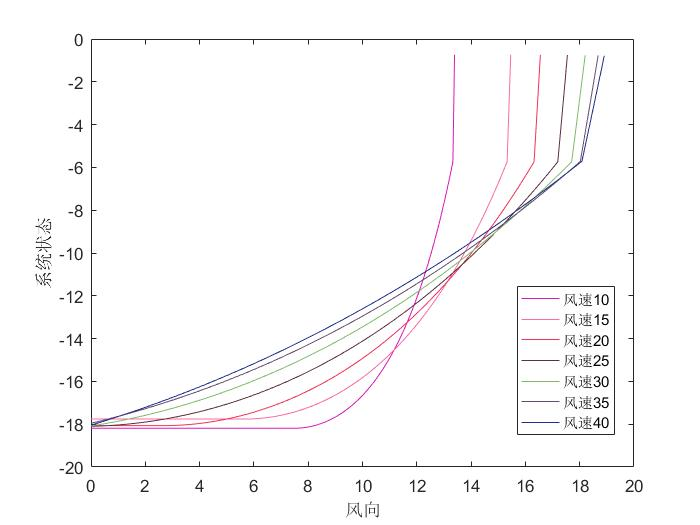
\includegraphics[width=\textwidth]{v_wind_effect_xitong.jpg}
                    \caption{风速对系泊系统的影响}
                    \label{风速对系泊系统的影响}
                \end{subfigure}
                \begin{subfigure}[b]{0.4\textwidth}
                    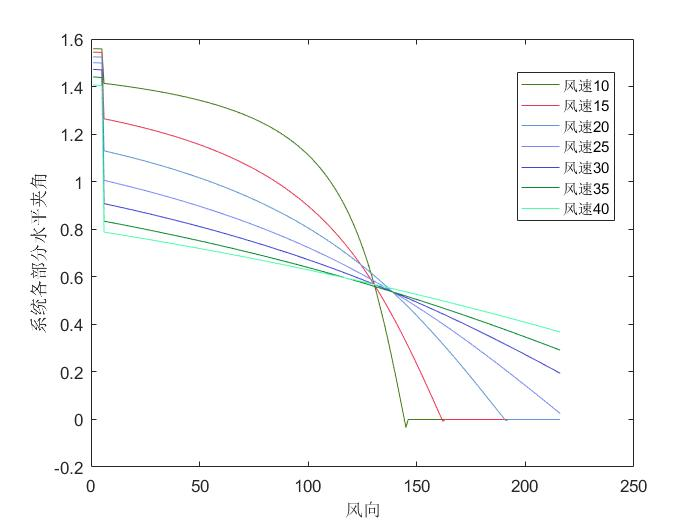
\includegraphics[width=\textwidth]{images/v_wind_effect_alpha2.jpg}
                    \caption{风速对系统水平夹角的影响}
                    \label{风速对系统水平夹角的影响}
                \end{subfigure}
                \caption{风速的敏感性分析}
            \end{figure}

    \subsection{改进一:含力矩平衡的系泊系统}
        \par
        在前面的建模部分,我们设计了2D系泊系统,并设计多目标优化模型来求解最优链型$I$、最优链长$L$和最优重物球质量$m_+$。下面,我们将用一种新的方法来设计2D系泊系统,并在此基础上进行优化设计。
        \subsubsection{模型建立与求解}
            \par
            在前面的系统受力分析当中,我们假设钢管(桶)的拉力方向是沿管方向的,并且没有考虑力矩平衡;我们还假设浮标适中竖直,不存在倾斜;并且在锚链的分析过程中,我们使用微元法对其进行分析;在2D系统中,我们并没有考虑海水流力的影响(假设海水静止)。下面,我们对整个系泊系统重新进行分析。
            \par
            \textbf{(1)建立二维直角坐标系}
            \par
            以锚为坐标原点,以风力方向为$x$轴正方向建立2维直角坐标系$xoy$,如图(\ref{系泊系统二维坐标系})所示
           \begin{figure}[H]
           \centering
           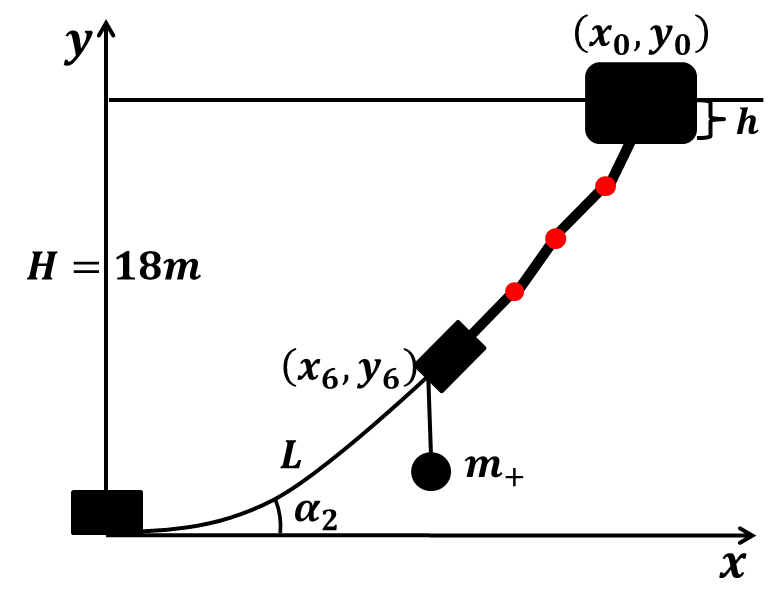
\includegraphics[height=4cm]{images/xiposystem_2_axis.jpg}
           \caption{系泊系统二维坐标系}
           \label{系泊系统二维坐标系}
           \end{figure}
            % \textcolor[rgb]{1 0 0}{todo:图片:系泊系统二维坐标系}\\
            在2D系泊系统中,我们假设海水流力与风力同向或反向,且各深度下海水流力相同。图(\ref{系泊系统二维坐标系})中$\alpha_2$为锚链底端水平夹角;$L$为锚链长度;$H$为海水深度;浮标底端接点坐标为$(x_0,y_0)$;锚链与钢桶交点坐标为$(x_6,y_6)$;$h = -y_0$为吃水深度;$m_+$为重物球质量;$w$为锚链单位重量。
            \par
            \textbf{(2)浮标受力分析}
            \par
            浮标受力分析如图(\ref{改进的浮标受力分析图})所示
            \begin{figure}[H]
            \centering
            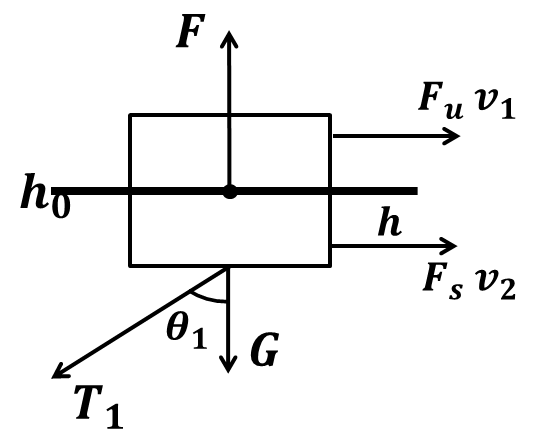
\includegraphics[height=3.5cm]{images/Improved_buoy_force_analysis_chart.jpg}
            \caption{改进的浮标受力分析图}
            \label{改进的浮标受力分析图}
            \end{figure}
            设$F_w$为风力,$F_s$为水流力,$F_w,F_s$方向相同,$v_1$为风速,$v_2$为水速,$h_0$为浮漂高,$G$为重力,$F$为浮力。浮标在$F_w,F_s,G,F,T$5力下处于静止平衡态,将浮标视为质点进行受力分析,有
            \begin{align*}
            & F_w = 0.625S_1 v_1^2 = 0.625 D(h_0-h)v_1^2\\
            & F_s = 374S_2 v_2^2 = 374 D hv_2^2\\
            & G = mg\\
            & F=\rho g v = \rho g\pi (D/2)^2h
            \end{align*}
            其中:$S_1$为浮标风力法平面投影;$S_2$为浮标海水流力法平面投影;$D$为浮标底直径。由静力平衡,有
            \begin{align*}
            & T_{x,1} = T\sin \theta = F_w+F_s\\
            & T_{y,1} = T\cos\theta = F_G
            \end{align*}
            \par
            \textbf{(3)钢管、钢桶受力分析}
            \par
            在进行受力分析之前,我们先引入力矩平衡。如图(\ref{力矩平衡示意图})所示
            \begin{figure}[H]
            \centering
            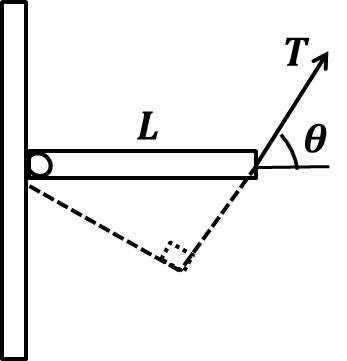
\includegraphics[height=3.5cm]{images/Moment_balance_diagram.jpg}
            \caption{力矩平衡示意图}
            \label{力矩平衡示意图}
            \end{figure}
            图(\ref{力矩平衡示意图})中的力臂为$L_T = L\sin \theta$,力矩为$M = F\cos\theta$。力矩平衡是指所有使物体顺时针转动的力矩之和等于所有使物体逆时针转动的力矩之和,即
            \begin{align*}
            \sum_i M_i = 0
            \end{align*}
            \par
            下面,我们来对钢管、钢桶进行受力分析,我们分两个方面:1.不考虑水流力$F_s$;2.考虑水流力$F_s$。
            \par
            (1)不考虑水流力$F_s$的影响。对第$i$节进行受力分析,受力分析如图(\ref{改进的钢管受力分析})
            \begin{figure}[H]
              \centering
              \begin{varwidth}[t]{\textwidth}
                \vspace{0pt}
                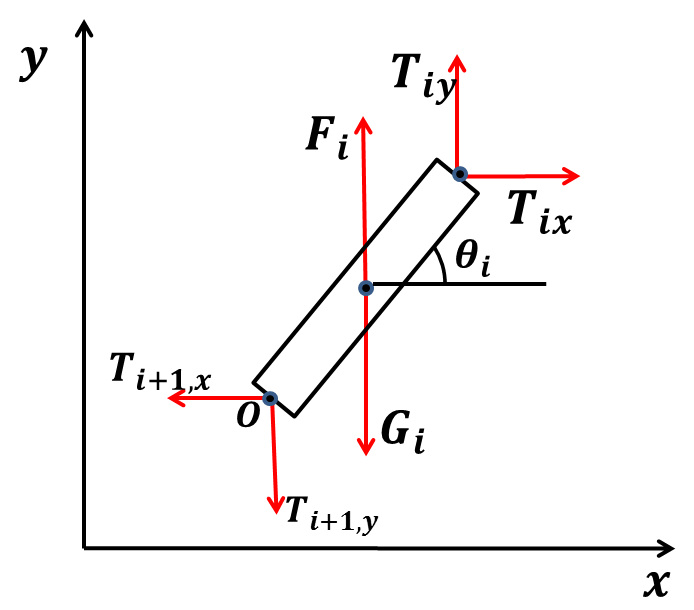
\includegraphics[height=4cm]{images/Improved_chart1.jpg}
              \end{varwidth}
              \qquad
              \begin{varwidth}[t]{\textwidth}
                \vspace{0pt}
                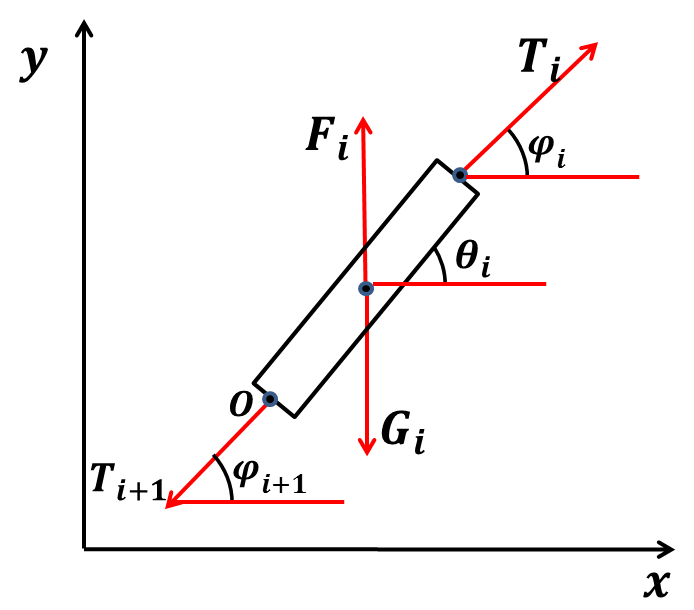
\includegraphics[height=4cm]{images/Improved_chart2.jpg}
              \end{varwidth}
            \caption{改进的钢管受力分析}
            \label{改进的钢管受力分析}
            \end{figure}
            其中:$o$为第$i$节的转动轴点,$G_i$为重力,$F_i$为浮力,$T_{ix},T_{iy}$为$T$的分量。如果不考虑海水流力$F_s$的影响,则$\forall i\in [1,2,3,\dots]$,有$T_{ix} = F_w$。
            \par
            第$i$节的受力平衡与力矩平衡为
            \begin{align*}
            & (G_i - F_i)\frac{l_i}{2}\cos\theta_i+T_{i,x}l_i\sin\theta_i = T_{i,y}l_i\cos\theta_i\\
            & T_{i,x} = T_{i+1,x}\\
            & T_{i,y} + F_i = G_i + T_{i+1,y}
            \end{align*}
            其中:$l$为钢管长。且注意,在研究钢桶受力分析时,$G_+ = m_+g$力矩为0。
            \par
            (2)考虑海水流力$F_s$的影响。钢管/钢桶的受力分析如图(\ref{改进的钢管受力分析-考虑海水流力})所示
            \begin{figure}[H]
            \centering
            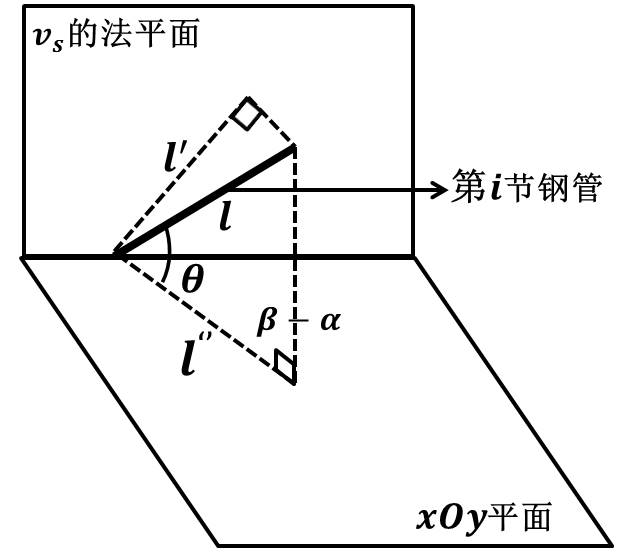
\includegraphics[height=4cm]{images/Steel_pipe_force_area.jpg}
            \caption{改进的钢管受力分析-考虑海水流力}
            \label{改进的钢管受力分析-考虑海水流力}
            \end{figure}
            对第$i$节受力分析时,考虑海水流力$F_{si}$的影响。受力平衡与力矩平衡为
            \begin{align*}
            & (G_i-F_i)\frac{l_i}{2}\cos\theta_i+T_{i,x}l_i\sin \theta_i+F_{s,i}\frac{l_i}{2}\sin \theta_i = T_{i,y}l_i\cos\theta_i\\
            & T_{i+1,x} = T_{i,x}+F_{s,i}\\
            & T_{i+1,y}+G_i = T_{i,y}+F_i
            \end{align*}
            其中:$F_{s,i}$为海水流力。下面,我们来计算各段的海水流力$F_{s,i} = 374S_i v_i^2$,$S_i$为第$i$节在水流力法平面上的投影,如图(\ref{钢管在水流力法平面上的投影示意图})所示
            \begin{figure}[H]
            \centering
            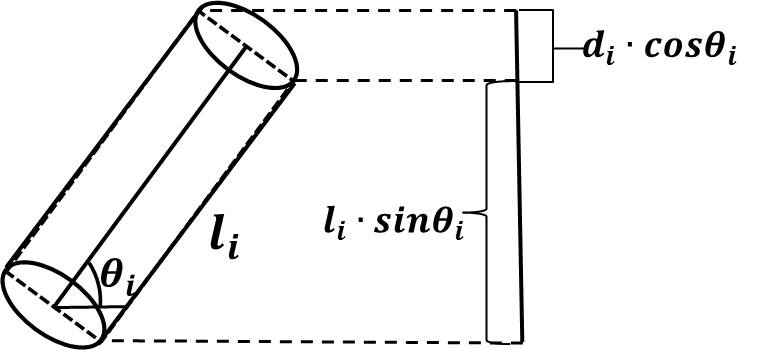
\includegraphics[height=3cm]{images/Pipe_projection.jpg}
            \caption{钢管在水流力法平面上的投影示意图}
            \label{钢管在水流力法平面上的投影示意图}
            \end{figure}
            \begin{align*}
            S_i = \left[ \frac{1}{2}\pi d_i\cos\theta_i+l_i\sin\theta_i \right]d_i
            \end{align*}
            其中:$d_i$为第$i$节底面直径。
            \par
            \textbf{(4)锚链分析}
            \par
            前面我们用微元法对锚链进行分析,下面,我们引入悬链线来分析锚链。锚链悬链线示意图如图(\ref{悬链线示意图})所示
            \begin{figure}[H]
            \centering
            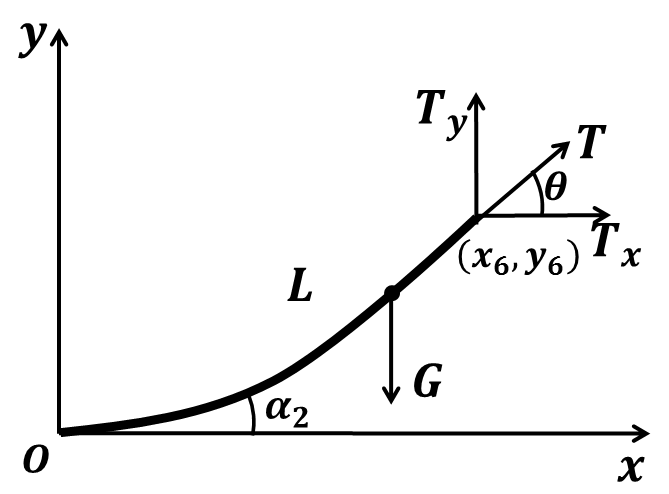
\includegraphics[height=4cm]{images/Catenary_line.jpg}
            \caption{悬链线示意图}
            \label{悬链线示意图}
            \end{figure}
            对于只受重力和两端拉力的链进行分析,设链处于平衡态,链下端顶点为$(0,0)$,末端顶点为$(x_6,y_6)$,下端水平夹角为$\alpha_2$。
            \par
            对悬链任意一微段$\mathrm{d}s$进行分析,有
            \begin{align*}
            \tan \theta = \frac{w\mathrm{d}s}{T_x}
            \end{align*}
            其中:$w$为链单位长度重量。而我们又知道$\tan\theta = \frac{\mathrm{d}y}{\mathrm{d}x}$,对其取微分,有
            \begin{align*}
            \mathrm{d}(\tan\theta) = \frac{w}{T_x}\mathrm{d}s = \frac{w}{T_x}\sqrt{(\mathrm{d}x)^2+(\mathrm{d}y)^2} = \frac{w}{T_x}\sqrt{1+\tan^2\theta}\mathrm{d}x
            \end{align*}
            对上式分离变量后积分,有
            \begin{align*}
            \int \frac{1}{\sqrt{1+\tan^2\theta}}\mathrm{d}(\tan\theta) = \int
            \frac{w}{T_x}\mathrm{d}x
            \end{align*}
            求解不定积分,有
            \begin{align*}
            & \sinh^{-1}(\tan\theta) = \frac{w}{T_x}x+C_1\\
            \Rightarrow{}& \tan\theta =  \sinh(\frac{w}{T_x}+C1) =\frac{\mathrm{d}y}{\mathrm{d}x}
            \end{align*}
            对上式再分离变量,有
            \begin{align*}
            \mathrm{d}y = \sinh(\frac{w}{T_x}x+C_1)\mathrm{d}x
            \end{align*}
            对上式求积分,有
            \begin{align*}
            y = \int \sinh(\frac{w}{T_x}x+C_1)\mathrm{d}x
            \end{align*}
            即
            \begin{align}
            \label{悬链线的一般方程}
            y =\frac{T_x}{w}\cosh(\frac{w}{T_x}x+C_1)+C_2
            \end{align}
            上式即为悬链线的一般方程,其中$C_1,C_2$为常数。
            \par
            下面,我们根据边值条件来求常数$C_1,C_2$。(1)求$C_1$:悬链末端水平夹角为$\alpha$,此为边值条件,于是我们对(\ref{悬链线的一般方程})式求导,有
            \begin{align*}
            y' = \sinh(\frac{w}{T_x}x+C_1)
            \end{align*}
            由$y'|_{x=0}=\tan\alpha$,有
            \begin{align*}
            C_1 = \ln (\tan\alpha+\sec\alpha)
            \end{align*}
            (2)求解$C_2$。由边值条件$y|_{x=0}=0$,有
            \begin{align*}
            C_2 = -\frac{T_x}{w}\sec\alpha
            \end{align*}
            故带参数$\alpha$的悬链线方程(\ref{悬链线的一般方程})具体为
            \begin{align*}
            y = \frac{T_x}{w}\cosh\left[\frac{w}{T_x}x+\ln (\tan\alpha+\sec\alpha) \right]-\frac{T_x}{q}\sec\alpha
            \end{align*}
            其中:$T_x,w$皆为已知量,$\alpha$为参数。
            \par
            \textbf{悬链线的长度$L$。}上面给出了锚链悬链线的带参方程,我们可以据此求出悬链线的长度$L$。先求微元段$\mathrm{d}s$
            \begin{align*}
            \mathrm{d}s = \sqrt{1+y^2}\mathrm{d}x = \cosh\left[ \frac{w}{T_x}x+\ln (\tan\alpha+\sec\alpha) \right]\mathrm{d}x
            \end{align*}
            将微元段$\mathrm{d}s$求和,有
            \begin{align*}
            S \triangleq L &= \oint \mathrm{d}s\\
            &=\frac{T_x}{w}\sinh \left[\frac{w}{T_x}x+\ln (\tan\alpha+\sec\alpha)  \right]+C_3
            \end{align*}
            由边值条件$S|_{x=0}=0$,有
            \begin{align*}
            C_3=-\frac{T_x}{w}\tan\alpha
            \end{align*}
            故带参数$\alpha$的悬链线长度方程为
            \begin{align*}
            S = \frac{T_x}{w}\sinh\left[ \frac{w}{T_x}x+\ln (\tan\alpha+\sec\alpha) \right]-\frac{T_x}{w}\tan\alpha
            \end{align*}
            \par
            \textbf{拉力$T$的计算}。悬链线拉力$T$的表达式为
            \begin{align*}
            T=T_x\sqrt{1+y^2}=T_x\cosh\left[ \frac{w}{T_x}x+\ln (\tan\alpha+\sec\alpha) \right]
            \end{align*}
            \par
            \textbf{(5)解非线性方程组求解系泊系统曲线}
            \par
            下面,我们来求解系泊系统曲线。系泊系统曲线是由$(x_6,h,\alpha)$三个参数决定的。求3个参数,要有三个方程,我们要求:\ding{172}海水深度为$18m$;\ding{173}锚链长度$L=22.05m$;\ding{174}力平衡。于是有如下非线性方程
            \begin{align}
            \label{系泊系统的非线性方程}
            &y_6  = H-h-\sum_{i=1}^5l\cos\theta_i=\frac{T_{x,6}}{w}\cosh\left[ \frac{w}{T_{x,6}}+\ln (\tan\alpha_2+\sec\alpha_2) \right]-\frac{T_x}{w}\sec\alpha_2\\
            &S \triangleq L = \frac{T_{x,6}}{w}\sinh\left[ \frac{w}{T_{x,6}}+\ln (\tan\alpha_2+\sec\alpha_2) \right]=22.05\\
            &T_{x,6}\cosh \left[\frac{w}{T_{x,6}}+\ln (\tan\alpha_2+\sec\alpha_2)\right]  = \sqrt{(T_{x,6})^6+(T_{y,6})^2}
            \end{align}
            其中:上面非线性方程中的第3个等式条件由下式变化而来
            \begin{align*}
            T = T_{x,6}\cosh\left[\frac{w}{T_{x,6}}+\ln (\tan\alpha_2+\sec\alpha_2)\right] = \sqrt{(T_{x,6})^6+(T_{y,6})^2}
            \end{align*}
            注意,上面方程组只有$h,x_6,\alpha$三个参数,其余量皆可用这三个量表示。解上述非线性方程组(\ref{系泊系统的非线性方程})可得到$(h,x_6,\alpha)$,即可得到整个系泊系统的情况。

        \subsubsection{程序}
            \par
            根据上述分析求解系泊系统,设置程序For2D.m如下
            \begin{lstlisting}[language = Matlab]
            function f = For2D_expand(xx, H, v1, v2, m_qiu, I, L, xitong_figure, xitong_save)
            %此函数是系泊系统的3元方程组的目标函数,用于fsolve函数。模型改进:引入"力矩平衡"和"悬链线方程"
            %
            %%%%输入%%%%
            % xx:y0,x0,alpha2。
            % v1:风速。
            % v2:水速。
            % H:海水深度。
            % m_qiu:重物球质量。
            % I:锚链型号。1、2、3、4、5
            % L:锚链长度。
            % xitong_figure:是否输入系统图像
            % xitong_save:是否保存系统数值结果
            %%%%正文%%%%
            y0 = xx(1);
            x0 = xx(2);
            alpha2 = xx(3);
            h = H - y0;
            y(1) = y0;
            x(1) = x0;
            %浮标受力
            rho = 1.025*10^3;%海水的密度  kg/m^3
            g = 9.8;%重力加速度 N/kg
            D = 2;%圆柱浮标地面直径 m
            h0 = 2;%圆柱浮标高度 m
            m0= 1000;%浮标质量 kg
            F0 = rho*g*pi*(D/2)^2*h;%浮标浮力
            G0 = m0*g;%浮标重力
            % v1 = 24;%风速 m/s
            % v2 = 1.5;%水速 m/s
            S_wind = D*(h0 - h);%风受力面积
            Fw = 0.625*S_wind*v1^2;%风力
            Fs0 = 374*D*h*v2^2;%海水流力
            Tx(1) = Fw + Fs0;
            Ty(1) = F0 - G0;
            %钢管受力
            for i = 1:4
                l(i) = 1;%钢管长度 m
                d(i) = 50/1000;%钢管直径 m
                m(i) = 10;%钢管质量 kg
                G(i) = m(i)*g;%钢管重力
                F(i) = rho*g*pi*(d(i)/2)^2*l(i);%钢管浮力
                %%%%参考:http://blog.sina.com.cn/s/blog_53f291190100cjss.html
                si = @(theta1)d(i)*(pi/2*d(i)*cos(theta1) + l(i)*sin(theta1));%第一根钢管的海水法平面投影
                Fsi = @(theta1)374*si(theta1)*v2^2;%第一根钢管的海水力
                fun = @(theta1)(G(i) - F(i))/2*cos(theta1) + Tx(i)*sin(theta1) + Fsi(theta1)*sin(theta1)/2 - Ty(i)*cos(theta1);
                theta1 = fsolve(fun, 0);
                theta(i) = theta1;
                Tx(i+1) = Tx(i) + Fsi(theta(i));
                Ty(i+1) = Ty(i) + F(i) - G(i);
                %钢管i的坐标(xi,yi)
                y(i+1) = y(i) - l(i)*sin(theta(i));
                x(i+1) = x(i) - l(i)*cos(theta(i));
            end
            %钢桶受力分析
            m_tong = 100;%钢桶的质量 kg
            G_tong = m_tong*g;%钢桶重力
            % m_qiu = 1200;%重物球质量 kg
            G_qiu = m_qiu*g;%重物球重力
            l_tong = 1;%钢桶长 m
            D_tong = 30/100;%钢桶底长
            F_tong = rho*g*pi*(D_tong/2)^2*l_tong;%钢桶浮力
            si = @(theta1)D_tong*(pi/2*D_tong*cos(theta1) + l_tong*sin(theta1));%第一根钢管的海水法平面投影
            Fsi = @(theta1)374*si(theta1)*v2^2;%第一根钢管的海水力
            fun = @(theta1)(G_tong - F_tong)/2*cos(theta1) + Tx(5)*sin(theta1) + Fsi(theta1)*sin(theta1)/2 - Ty(5)*cos(theta1);
            theta_tong = fsolve(fun, 0);
            theta(5) = theta_tong;
            Tx(6) = Tx(5) + Fsi(theta(5));
            Ty(6) = Ty(5) + F_tong - G_tong - G_qiu;
            y(6) = y(5) - l_tong*sin(theta(5));
            x(6) = x(5) - l_tong*cos(theta(5));
            %确定锚链
            switch I
                case 1
                   II = 78/1000;%锚链每节长度 m
                   m_II = 3.2;%单位长度的质量 kg/m
                case 2
                   II = 105/1000;%锚链每节长度 m
                   m_II = 7;%单位长度的质量 kg/m
                case 3
                   II = 120/1000;
                   m_II = 12.5;%单位长度的质量 kg/m
                case 4
                    II = 150/1000;
                    m_II = 19.5;%单位长度的质量 kg/m
                case 5
                    II = 180/1000;
                    m_II = 28.12;%单位长度的质量 kg/m
            end
            n = floor(L/II);
            % L = 22.05;
            w = m_II*g;
            f(1) = Tx(6)/w*cosh(w/Tx(6)*x(6) + log(tan(alpha2) + sec(alpha2))) - Tx(6)/w*sec(alpha2)...
                - y0 + l(1)*sin(theta(1)) + l(2)*sin(theta(2)) + l(3)*sin(theta(3)) + l(4)*sin(theta(4))...
                 + l_tong*sin(theta(5));
            f(2) = Tx(6)/w*sinh(w/Tx(6)*x(6) + log(tan(alpha2) + sec(alpha2))) - Tx(6)/w*tan(alpha2)...
                - L;
            f(3) = Ty(6)/Tx(6) - sinh(w/Tx(6)*x(6) + log(tan(alpha2) + sec(alpha2)));
            \end{lstlisting}
            求解非线性方程组(\ref{系泊系统的非线性方程})
            \begin{lstlisting}[language = Matlab]
            function bestxx = bestpoint3_expand(H, v1, v2, m_qiu, I, L, xitong_figure, xitong_save)
            %此函数用于求解系泊系统的3元方程组,从而求出最优y0,x0,alpha2。
            %
            %%%%正文%%%%
            fun = @(xx)For2D_expand(xx, H, v1, v2, m_qiu, I, L, xitong_figure, xitong_save);
            xx0 = [H-0.7, 20, 0];
            bestxx = fsolve(fun, xx0);
            end
            \end{lstlisting}
        \subsubsection{结果}
            \par
            风速$v=36m/s$时(风速12/24时存在错误,锚链拖尾状态没有处理好),改进的系泊系统图像如图(\ref{风速36、吃水深度0.770003时的系统系统(改进)})所示
            \begin{figure}[H]
                \centering
                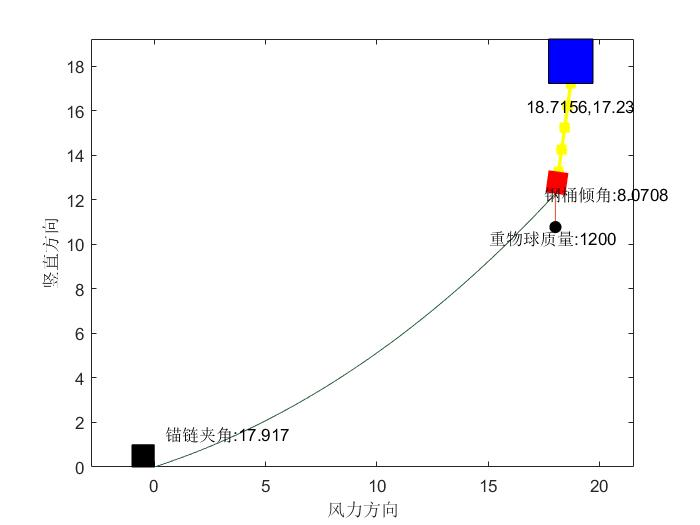
\includegraphics[width=8cm]{images/v_wind_36_h_xitong_gaijin.jpg}
                \caption{风速36、吃水深度0.770003时的系统系统(改进)}
                \label{风速36、吃水深度0.770003时的系统系统(改进)}
            \end{figure}
            \par
            下面给出水深$H$、水速$v_2$对系统的影响(敏感性分析)。水深$H$、水速$v_2$对系统的影响如图(\ref{水深、水速的敏感性分析})所示
            \begin{figure}[H]
                \centering
                \begin{subfigure}[b]{0.4\textwidth}
                    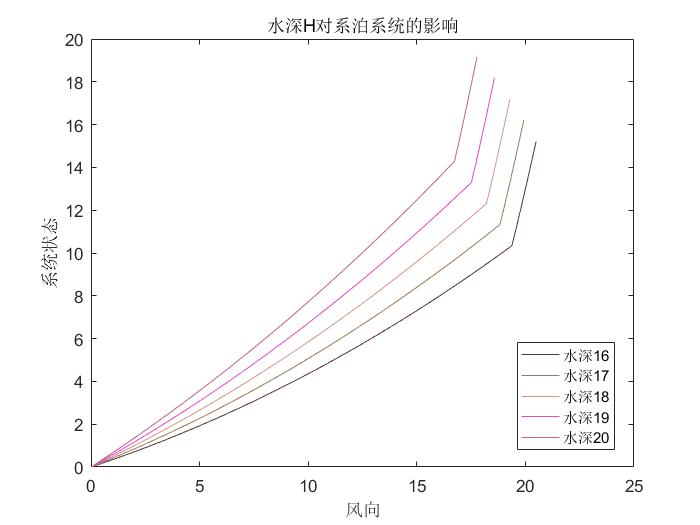
\includegraphics[width=\textwidth]{images/H_effect_xitong.jpg}
                    \caption{水深H的灵敏度分析}
                    \label{水深H的灵敏度分析}
                \end{subfigure}
                \begin{subfigure}[b]{0.4\textwidth}
                    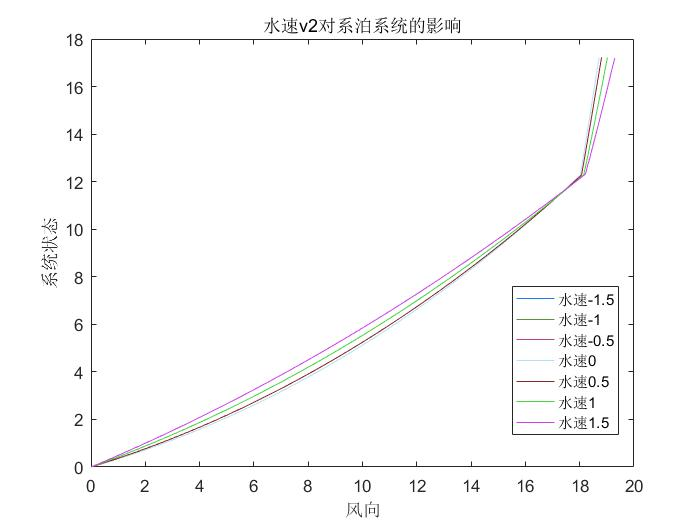
\includegraphics[width=\textwidth]{images/v2_effect_xitong.jpg}
                    \caption{水速v2的灵敏度分析}
                    \label{水速v2的灵敏度分析}
                \end{subfigure}
                \caption{水深、水速的敏感性分析}
                \label{水深、水速的敏感性分析}
            \end{figure}

    \subsection{改进二:3维坐标系下的系泊系统}
        \par
        上面的系泊系统是在二维平面$xoy$下进行分析的,并没有考虑到强水速$v_s$。如果海水流速较强,则系泊系统的状态应该是一个三维空间的曲线,为此,我们建立三维空间$xyzo$下的系泊系统,并进行相应的受力分析。
        \subsubsection{三维系泊系统建立}
            \par
            \textbf{(1)建立空间直角坐标系}
            \par
            我们先固定水深$H_s=18m$,海水流速 $v_s=1.5m/s$,风速$v_w =24m/s$,设风速$v_w$与海水流速$v_s$所成的夹角为$\beta=90^\circ$,以风力$F_w$所在的方向为$y$轴正向,以垂直海平面向上的方向为$z$轴正方向,建立如图(\ref{海中某点在三维空间中受力示意图})所示的空间直角坐标系。
            \begin{figure}[H]
            \centering
            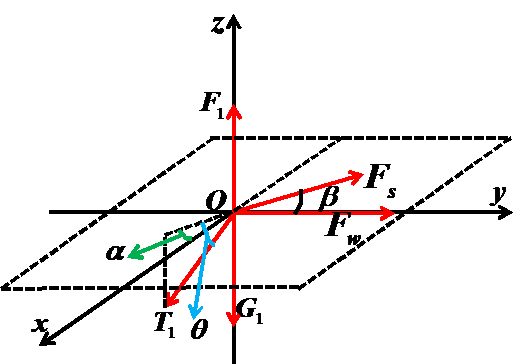
\includegraphics[height=4cm]{images/onepoint_force_analysis_in_sea.jpg}
            \caption{海中某点在三维空间中受力示意图}
            \label{海中某点在三维空间中受力示意图}
            \end{figure}
            \par
            \textbf{(2)浮标受力分析}
            \par
            假设浮标在风力和水流力的作用下仍保持水平。对浮标进行受力分析,如图(\ref{浮标三维受力分析})所示。
            \begin{figure}[H]
            \centering
            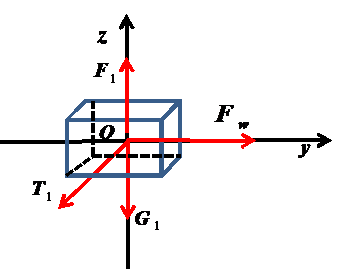
\includegraphics[height=4cm]{images/buoy_three_dimensions_force_analysis.jpg}
            \caption{浮标三维受力分析}
            \label{浮标三维受力分析}
            \end{figure}
            \par
            在三维坐标空间对浮标进行受力分析,浮标受到的力有重力$G_1$、浮力$F_1$、第一根钢管对它的拉力$T_1$、风力$F_w$、近海水流力$F_s$。设浮标的吃水深度为$h$,拉力与平面的夹角为$\theta$,与$x$轴的夹角为$\alpha$,$\beta$为水流的方向与$y$轴正方向的夹角。
            类似问题一中浮标的受力分析可得浮标所受的重力、浮力、风力、水流力分别为(单位:N):
            \begin{align*}
            & G_0 = m_0g\\
            & F_0 = \rho g\pi ( D/2 )^2h\\
            & F_s = 374Dhv_s^2\\
            & F_w = 0.625D(h_0-h)v_w^2
            \end{align*}
            其中:$m_0$为浮标的质量,$\rho$为海水密度,$D$为浮标的底面直径,$h_0$为浮标高度,$h$为吃水深度,$v_w$为海面风速,$v_s$为水流速度。
            \par
            第一张力$T_1$在各个方向的大小分别如下
            \begin{align*}
            & T_{1x} = T_1\cos\theta_1\cos\alpha_1\\
            & T_{1y} = T_1\cos\theta_1\sin\alpha_1\\
            & T_{1z} = T_1\sin \theta_1
            \end{align*}
            浮标在水中最终处于静力平衡状态,得到静力平衡方程组
            \begin{align*}
            & T_{1x} = F_s\sin \beta\\
            & T_{1y} = F_w + F_s\cos\beta\\
            & T_{1z} + G_1 = F_1
            \end{align*}
            \par
            上述方程组中通过先给定浮标的吃水深度$h$,可得到$F_s,F_w,F_1$的值而可求得,$T_1,\alpha_1,\theta_1$的值。进一步,在已知钢管长度$l$为$1m$的情况下,利用静力平衡方程的结果得到第一根钢管的下端点的坐标$(x_2,y_2,z_2)$如下
            \begin{align*}
            & x_2 = l\cos\theta_1\cos\alpha_1+x_1\\
            & y_2 = l\cos\theta_1\sin\alpha_1+y_1\\
            & z_2 = l\sin\theta_1+z_1
            \end{align*}
            其中,$(x_1,y_1,z_1)$为浮标与钢管连接处的坐标。
            \par
            \textbf{(3)钢管受力分析}
            \par
            水中钢管的受力情况如图(\ref{水中钢管受力示意图})所示
            \begin{figure}[H]
            \centering
            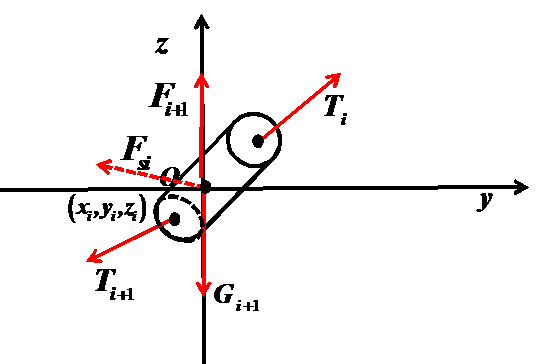
\includegraphics[height=4cm]{images/water_pipe_force.jpg}
            \caption{水中钢管受力示意图}
            \label{水中钢管受力示意图}
            \end{figure}
            \par
            与前面的分析相同,第$i$ 根钢管受到的力有重力$G_{i+1}$、浮力$F_{i+1}$、钢管受到的前端拉力与后端拉力分别为$T_i$和$T_{i+1}$ 、近海水流力$F_{si}$, 为钢管的数量。下面,我们来推到近海水流力$F_{si}$的计算,$F_{si} = 374Sv_s^2$,因此,我们只要求出每节钢管在海里的受力面积即可,钢管的投影如图(\ref{钢管受力面积分析图})所示
            \begin{figure}[H]
            \centering
            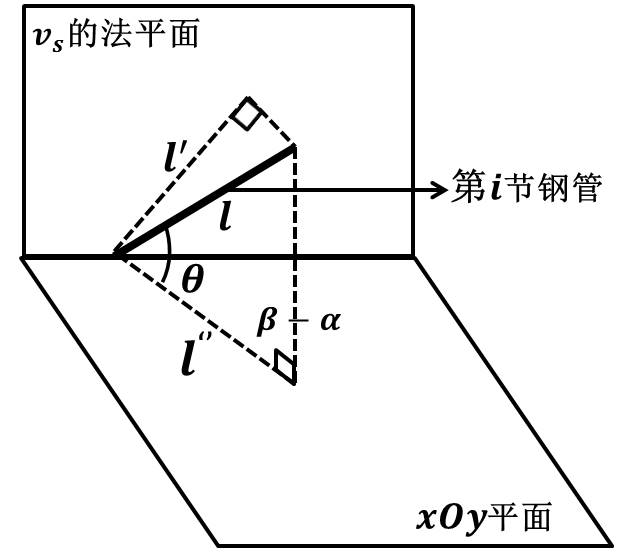
\includegraphics[height=4cm]{images/Steel_pipe_force_area.jpg}
            \caption{钢管受力面积分析图}
            \label{钢管受力面积分析图}
            \end{figure}
            可以推得
            \begin{align*}
            l' =&  \sqrt{[l\cos\theta\cos(\beta-\alpha)]^2+(l\sin\theta)^2}\\
            =& l\sqrt{\cos^2\theta\cos^2(\beta-\alpha)+\sin^2\theta}
            \end{align*}
            而且$S = dl'$,所以
            \begin{align*}
            F_{si} =&  374S v_s^2\\
            =& 374dl\sqrt{\cos^2\theta\cos^2(\beta-\alpha)+\sin^2\theta}v_s^2
            \end{align*}
            $d$为钢管直径,$d,l,\beta$均为定值,$F_{si}$为第$i$根钢管在平衡状态下受到的水流力,得到钢管的静力平衡方程组如下
            \begin{align*}
            & T_{ix} = T_i\cos\theta_i\cos\alpha_i\\
            & T_{iy} = T_i\cos\theta_i\sin\alpha_i\\
            & T_{iz} = T_i\sin\theta_i
            \end{align*}
            其中,$T_{ix},T_{iy},T_{iz}$ 分别为张力$T_i$在$x$轴、$y$轴、$z$轴方向的分力,$\beta$为水流的方向与y轴正方向的夹角。求解上述静力平衡方程,可以得到$T_{i+1},\theta_{i+1},\alpha_{i+1}$。由此得到关于第$i$根钢管的下端坐标的方程组
            \begin{align*}
            & x_{i+1} = l\cos\theta_{i+1}\cos\alpha_{i+1}+x_i\\
            & y_{i+1} = l\cos\theta_{i+1}\sin\alpha_{i+1}+y_i\\
            & z_{i+1} = l\sin \theta_{i+1}+z_i
            \end{align*}

            \par
            \textbf{(4)钢桶的受力分析}
            \par
            将钢桶与重物球看成一个整体进行受力分析,如图(\ref{钢桶与重物球的受力示意图})所示
            \begin{figure}[H]
            \centering
            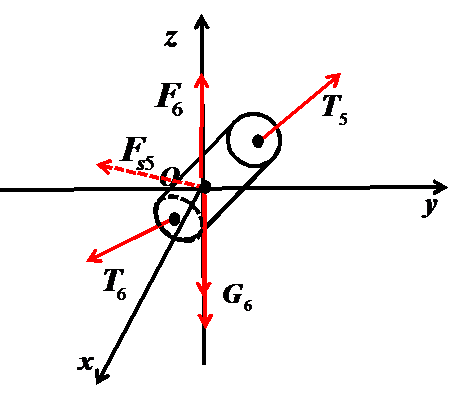
\includegraphics[height=4cm]{images/Steel_pipe_and_weight_ball_force.jpg}
            \caption{钢桶与重物球的受力示意图}
            \label{钢桶与重物球的受力示意图}
            \end{figure}
            \par
            与第一问类似,钢桶和重物球受到的力有重力$G_5$和$G_6$ 、浮力$F_5$、海水流力$F_{s5}$、上端与下端的拉力分别为$T_5$和$T_6$。根据钢桶和重物球处于平衡状态,得到钢桶和重物球的静力平衡方程如下
            \begin{align*}
            & T_{6x} = T_{5x}+F_{s5}\sin \beta\\
            & T_{6y} = T_{5y}+F_{s5}\cos \beta\\
            & T_6 + G_5+G_6 = F_5+T_{5z}
            \end{align*}
            \par
            \textbf{(5)对锚链进行分析}
            \par
            方法1:假设锚链形状可改变但没有弹性,类比于我们在问题一种分析的那样,利用微元法对锚链的微段$\mathrm{d}s$进行受力分析。求解各段$T_i$、$\theta_i$ 、$\alpha_i$ 、$(x_i,y_i,z_i)$ 的迭代公式,但这些迭代公式表示复杂,求解较麻烦。这种方法用到了微元法,我们并没有求解出来。故而选取了下面的方法2。
            \par
            方法2:考虑锚链是环环相扣的环链(这种情况符合本文题设条件中锚链是无档普通链环的情况)。设锚链共有$n$节环,由问题一可知锚链在水中受到的浮力相对于重力而言可忽略不计。因此我们可以得到第 节连环$T_i$、$\theta_i$ 、$\alpha_i$ 、$(x_i,y_i,z_i)$的迭代公式(可与之前类似推得)。
        \subsubsection{程序}
            \par
            三维空间中的系泊系统求解程序For3D如下
            \begin{lstlisting}[language = Matlab]
            function [z, y, x, theta, alpha, T, stat] = For3D(z0, y0, x0, v1, v2, m_qiu, I, L, beta, xitong_figure)
            % 此函数用于给定x0、y0和z0后求解3D系泊系统的状态曲线
            %%%%正文%%%%
            h = abs(z0);
            %确定锚链
            switch I
                case 1
                   II = 78/1000;%锚链每节长度 m
                   m_II = 3.2;%单位长度的质量 kg/m
                case 2
                   II = 105/1000;%锚链每节长度 m
                   m_II = 7;%单位长度的质量 kg/m
                case 3
                   II = 120/1000;
                   m_II = 12.5;%单位长度的质量 kg/m
                case 4
                   II = 150/1000;
                   m_II = 19.5;%单位长度的质量 kg/m
                case 5
                   II = 180/1000;
                   m_II = 28.12;%单位长度的质量 kg/m
            end
            n = round(L/II);
            ind = n+5+1;

            %浮标、钢管分析
            fun = @(x_point)(D3fun_fubiao(x_point, beta, z0, v1, v2));
            X0 = [14000, 0, pi/2];%T1、theta1和alpha1的初始搜索点
            [x_solve, ~] = fsolve(fun, X0);
            T(1) = x_solve(1);
            theta(1) = x_solve(2);
            alpha(1) = x_solve(3);
            x(1) = x0;
            y(1) = y0;
            z(1) = z0;
            for i = 1:4
                l = 1;%钢管长度
                Ti = T(i);
                thetai = theta(i);
                alphai = alpha(i);
                fun = @(x_point)(D3fun_gangguan(x_point, Ti, thetai, alphai, beta, v2));
                X0 = [Ti, thetai, alphai];%T、theta和alpha的初始搜索点
                [x_solve, ~] = fsolve(fun, X0);
                T(i+1) = x_solve(1);
                theta(i+1) = x_solve(2);
                alpha(i+1) = x_solve(3);
                if alpha(i) < pi/2
                    x(i+1) = x(i) + l*cos(theta(i))*cos(alpha(i));
                else
                    x(i+1) = x(i) - l*cos(theta(i))*cos(alpha(i));
                end
                y(i+1) = y(i) - l*cos(theta(i))*sin(alpha(i));
                z(i+1) = z(i) - l*sin(theta(i));
            end
            %钢桶分析
            l_tong = 1;%钢桶长 m
            T5 = T(5);
            theta5 = theta(5);
            alpha5 = alpha(5);
            fun = @(x_point)(D3fun_gangtong(x_point, T5, theta5, alpha5, beta, v2, m_qiu));
            X0 = [T5, theta5, alpha5];
            [x_solve, ~] = fsolve(fun, X0);
            T(6) = x_solve(1);
            theta(6) = x_solve(2);
            alpha(6) = x_solve(3);
            if alpha(5) < pi/2
                x(6) = x(5) + l_tong*cos(theta(5))*cos(alpha(5));
            else
                x(6) = x(5) - l_tong*cos(theta(5))*cos(alpha(5));
            end
            y(6) = y(5) - l_tong*cos(theta(5))*sin(alpha(5));
            z(6) = z(5) - l_tong*sin(theta(5));
            %锚链线分析
            L_tuo = 0;%锚链拖尾长度
            for i = 6 : 6+n-1
                if  theta(i) - 0 >0.001
                    Ti = T(i);
                    thetai = theta(i);
                    alphai = alpha(i);
                    fun = @(x_point)(D3fun_maolian(x_point, Ti, thetai, alphai, I));
                    X0 = [Ti, thetai, alphai];%T、theta和alpha的初始搜索点
                    [x_solve, ~] = fsolve(fun, X0);
                    T(i+1) = x_solve(1);
                    theta(i+1) = x_solve(2);
                    alpha(i+1) = x_solve(3);
                    if alpha(i) < pi/2
                        x(i+1) = x(i) + II*cos(theta(i))*cos(alpha(i));
                    else
                        x(i+1) = x(i) - II*cos(theta(i))*cos(alpha(i));
                    end
                    y(i+1) = y(i) - II*cos(theta(i))*sin(alpha(i));
                    z(i+1) = z(i) - II*sin(theta(i));
                else
                    T(i+1) = 0;
                    theta(i+1) = 0;
                    alpha(i+1) = alpha(i);

                    z(i+1) = z(i);
                    y(i+1) = y(i) - II*sin(alpha(i));
                    if alpha(i) < pi/2
                        x(i+1) = x(i) + II*cos(alpha(i));
                    else
                        x(i+1) = x(i) - II*cos(alpha(i));
                    end
                    L_tuo = L_tuo+II;
                end
            end
            \end{lstlisting}
            \par
            在求解$T_i,\theta_i,\alpha_i$的方程组时,要注意这个方程组会有两个解,我们要选择合适的。上面的程序中用到了D3fun$\_$fubiao.m,D3fun$\_$gangguan.m,D3fun$\_$gangtong.m和D3fun$\_$maolian.m,这里我们仅给出D3fun$\_$gangguan.m的程序,其余相似
            \begin{lstlisting}[language = Matlab]
            function y = D3fun_gangguan(x_point, T, theta, alpha, beta, v2)
            %此函数用于求解钢管的T、theta和alpha
            %
            %%%%%输入说明%%%%
            % x:解。T,theta,alpha
            % T:Ti-1
            % theta:
            %%%%正文%%%%
            Tx = T*cos(theta)*cos(alpha);
            Ty = T*cos(theta)*sin(alpha);
            Tz = T*sin(theta);
            %钢管受力分析
            rho = 1.025*10^3;
            g = 9.8;
            m = 10;%钢管质量 kg
            G = m*g;%钢管重力
            l = 1;%钢管长度 m
            d = 50/1000;%钢管直径 m
            F = rho*g*pi*(d/2)^2*l;%钢管浮力
            % s = d*(l^2 - l^2*(cos(theta))^2*(sin(alpha-beta))^2);
            s = d*l*sqrt((cos(theta))^2*(cos(beta - alpha))^2 + (sin(theta))^2);
            Fs = 374*s*v2^2;
            Ti = x_point(1);
            thetai = x_point(2);
            alphai = x_point(3);
            Tix = Ti*cos(thetai)*cos(alphai);
            Tiy = Ti*cos(thetai)*sin(alphai);
            Tiz = Ti*sin(thetai);
            y = [Tix - Tx - Fs*sin(beta);...
                Tiy - Fs*cos(beta) - Ty;...
                Tiz + G - F - Tz];
            end
            \end{lstlisting}

        \subsubsection{结果}
            \par
            风速$v=12m/s$时的锚链末端$z_n$和水平面夹角$\theta$随吃水深度$h$的变化曲线如图(\ref{风速12时锚链末端及水平面夹角随吃水深度h的变化曲线})所示。
            \begin{figure}[H]
                \centering
                \begin{subfigure}[b]{0.4\textwidth}
                    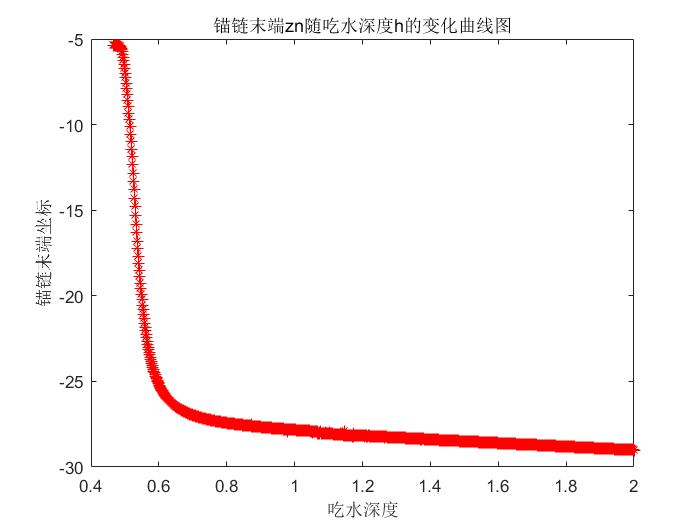
\includegraphics[width=\textwidth]{images/3D_v_wind_12_zn_h.jpg}
                    % \caption{3D系统锚链末端zn随吃水深度h的变化}
                \end{subfigure}
                \begin{subfigure}[b]{0.4\textwidth}
                    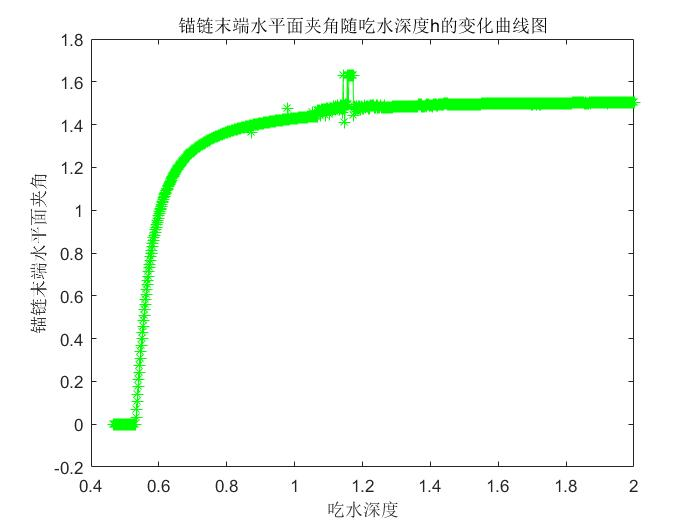
\includegraphics[width=\textwidth]{images/3D_v_wind_12_theta_h.jpg}
                    % \caption{3D系统水平面夹角theta随吃水深度h的变化}
                \end{subfigure}
                \caption{风速12时锚链末端及水平面夹角随吃水深度h的变化曲线}
                \label{风速12时锚链末端及水平面夹角随吃水深度h的变化曲线}
            \end{figure}
            在最优吃水深度下,风速$v_w=24m/s$时系泊系统的3D系统曲线如图(\ref{风速12、吃水深度0.54107时的3D系泊系统})所示。
            \begin{figure}[H]
                \centering
                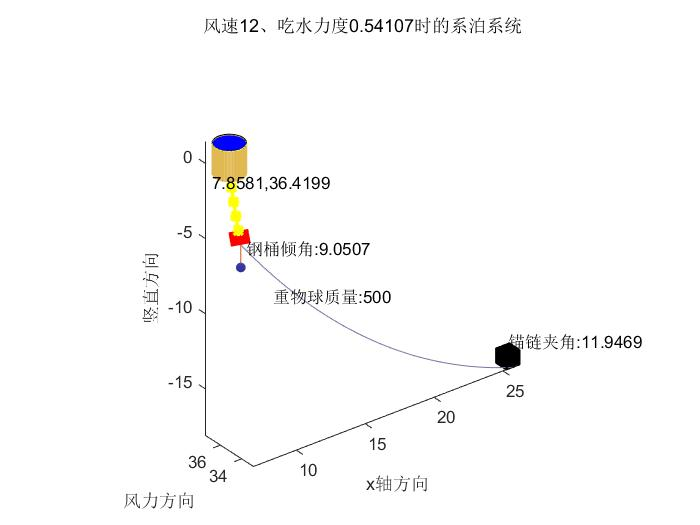
\includegraphics[width=8cm]{images/3D_v_wind_12_h_xitong.jpg}
                \caption{风速12、吃水深度0.54107时的3D系泊系统}
                \label{风速12、吃水深度0.54107时的3D系泊系统}
            \end{figure}
            % \par
            % 风速$v=24m/s$时的系统
            % \par
            % 风速$v=36m/s$时的系统

    \subsection{总结}
        \par
        1.建模过程不要急躁。由于在编程时的一点失误(括号没对齐),我们差一点就放弃了。遇到程序问题,把程序打印下来,一行一行的捋,慢慢来,别着急。
        \par
        2.这种题型的一般题目要求是:第一问,寻找变量之间的关系;第二问,设计优化模型,来达到某种要求;第三问,敏感性分析。当然,也没有必要循规蹈矩,你想怎样做就怎样做,没关系。

% \bibliography{}%bib文件名称
\end{document}
